\documentclass[%
    school=etsisi,%
    type=pfg,%
    degree=61IW,%
]{upm-report}

\setcounter{tocdepth}{1} % para ver si se incluyen subsecciones o no cambiar el depthde 1 a 2

\newcommand{\elvi}[2][inline]{\color{violet} [EAD]: #2\color{black}}

\usepackage[dvipsnames]{xcolor}


%%%%%%%%%%%%%%%%%%%%%%%%%%%%%%%%%%%%%%%%%%%%%%%%%%%%%%%%%%%%%%%%%%%%%%%%
% TÍTULO, AUTORES Y DIRECTORES
%
\title{PANOT: Plataforma Móvil para la Gestión de las Relaciones Personales mediante la captura asistida de Interacciones}
\author{Ángel Rodríguez Morán}
\bibauthor{}
\director{Elvira Amador Domínguez}

%%%%%%%%%%%%%%%%%%%%%%%%%%%%%%%%%%%%%%%%%%%%%%%%%%%%%%%%%%%%%%%%%%%%%%%%
% RESUMEN Y ABSTRACT
%
\abstract{spanish}{
    Este Proyecto Fin de Grado presenta el análisis, diseño, desarrollo y lanzamiento de PANOT, una plataforma móvil que tiene como objetivo ser una extensión cognitiva para la gestión de las 
    relaciones personales. El objetivo principal es construir un Producto Mínimo Viable para habilitar la validación de si es posible reducir 
    la carga cognitiva del usuario en la gestión de sus relaciones personales mediante el registro de interaciones y el uso de Inteligencia Artificial. 
    Para alcanzar este propósito, se ha implementado una metodología basada en el Libro de Eric Ries \textit{The Lean Startup}, en que la evolución de un producto se apoya en 
    el ciclo de \textit{Construir-Medir-Aprender}. La solución técnica destaca por una arquitectura \textit{local-first} que garantiza la operatividad de las funcionalidades principales en modo offline, 
    apoyada en una insfraestructura alojada en la plataforma Supabase. El módulo de procesamiento semántico utiliza un motor multi-agente desarrollado con LangChain que extrae entidades y relaciones de forma automatizada a 
    través de una interfaz \textit{voice-first}. Este enfoque da la posibilidad al usuario de capturar información relevante sobre sus contactos mediante notas de voz, 
    eliminando la fricción de la entrada manual de datos.

    Los resultados obtenidos confirman la factibilidad técnica y económica de la propuesta. El sistema es capaz de procesar interacciones complejas con una latencia media y 
    un coste operativo asumibles. Además, se ha verificado el éxito del matching semántico, permitiendo al sistema descubrir conexiones no evidentes entre contactos de forma autónoma. 
    El proyecto culmina con el despliegue real de la aplicación en la App Store de Apple, superando sus auditorias de privacidad y diseño, y la publicación del lanzamiento en la plataforma Product Hunt.

}
\keywords{spanish}{
    Aplicación Móvil para iOS, Interfaz por voz, Inteligencia Relacional, Grafos de Conocimiento, Sistema Multi-Agente, Arquitectura local-first 
}

\abstract{english}{
    The project presents the analisys, design, development y launch of PANOT, a mobile platform that aims to be a cognitive extension for the user's personal relationship management. The main objective 
    is to build a Minimum Viable Product to be able to validate if it is possioble to reduce the cognitive load of users in the management of his personal relationships by laveraging the capture of their interactions 
    and Artificial Intelligence. To achive this purpose, a methodology based on the book of Eric Ries \textit{The Lean Startup} has been implemented, in which the evolution of a product is supported by the 
    cycle of \textit{Build-Measure-Learn}. The technical solution features a \textit{local-first} architecture that ensures the operability of core functionalities in offline mode, supported by an infrastructure 
    hosted on the Supabase platform. The semantic processing module utilises a multi-agent engine developed in LangChain, which automatically extracts entities and relationships through a \textit{voice-first} interface. 
    This approach gives the enables users to capture relevant information regarding their contacts via voice notes, eliminating the friction associated with manual data entry.
    
    The obteined results confirm the technical and economic feasibility of the proposal. The system is capable of processing complex text-based interactions with acceptable average latency and operating costs. 
    Furthermore, the success of the semantic mathing has been verified, allowing the system to autonomously discover non-obvious connections between contacts. The project culminates with the actual deployment 
    of the application on the Apple's App Store, successfully passing the privacy and design audits, and the launch on the Product Hunt platform.

}
\keywords{english}{
    Mobile application for iOS, Voice interface, Relational Intelligence, Knowledge Graphs, Multi-Agent System, Local-first architecture
}

% Opcional
\reportquotation{
    Create the things you wish existed.
}{Unknown}

% Opcional
\acknowledgements{
    [Escribir aquí los agradecimientos del proyecto]
}

%%%%%%%%%%%%%%%%%%%%%%%%%%%%%%%%%%%%%%%%%%%%%%%%%%%%%%%%%%%%%%%%%%%%%%%%
% GLOSARIO Y ABREVIATURAS
%
% Añadir aquí las entradas del glosario y acrónimos necesarios para el proyecto
\newglossaryentry{inferencia-analogica}{
        name=Inferencia Analógica,
        description={
            Transmisión de conocimientos de una situación a otra.
        }
}
\newglossaryentry{generalizacion-de-cero-disparos}{
        name=Generalización de Cero Disparos,
        description={
            Escenario de aprendizaje automático en el que se entrena un modelo de IA para reconocer y categorizar 
            objetos o conceptos sin haber visto ningún ejemplo de esas categorías o conceptos de antemano.
        }
}

\newglossaryentry{aes-256}{
        name=AES-256,
        description={
            Estándar de Cifrado Avanzado (Advanced Encryption Standard) que utiliza una longitud de clave de 256 bits. 
            Es uno de los algoritmos de cifrado simétrico más seguros y utilizados actualmente para proteger información 
            clasificada y datos sensibles.
        }
}

\newglossaryentry{transport-layer-security}{
        name=Transport Layer Security,
        description={
            Protocolo de seguridad que proporciona autenticación, integridad y confidencialidad de los datos en tránsito 
            entre dos puntos, generalmente entre un cliente y un servidor.
        }
}

\newglossaryentry{row-level-security}{
        name=Row Level Security,
        description={
            Mecanismo de seguridad que permite controlar el acceso a las filas de una tabla de base de datos según el usuario 
            que realiza la consulta.
        }
}

\newglossaryentry{column-level-security}{
        name=Column Level Security,
        description={
            Mecanismo de seguridad que permite controlar el acceso a las columnas de una tabla de base de datos según el usuario 
            que realiza la consulta.
        }
}

\newglossaryentry{soc-2-type-2}{
        name=SOC 2 Type 2,
        description={
            Estándar de auditoría desarrollado por el AICPA (Instituto Americano de Contadores Públicos Certificados) que 
            revisa y verifica tanto el diseño como el funcionamiento efectivo de los controles de seguridad implementados 
            por una organización para salvaguardar los datos de sus clientes durante un intervalo determinado, generalmente 
            comprendido entre 3 y 12 meses.
        }
}

\newglossaryentry{analisis-cohorte}{
        name=Análisis de Cohorte,
        description={
            Técnica de análisis de datos que divide a un grupo de individuos en subgrupos basados en características comunes 
            y observa cómo evolucionan estos individuos a lo largo del tiempo.
        }
}

\newglossaryentry{embudos}{
        name=Embudos,
        description={
            Técnica de análisis de datos que permite visualizar cómo los usuarios interactúan con diferentes partes de un producto 
            a lo largo del tiempo, ayudando a identificar patrones de retención y conversión.
        }
}

\newglossaryentry{construir-medir-aprender}{
        name=Construir-Medir-Aprender,
        description={
            Ciclo de retroalimentación fundamental de la metodología \textit{Lean Startup} diseñado para transformar ideas en productos (Construir), 
            evaluar la reacción de los clientes mediante datos (Medir) y validar o refutar hipótesis para decidir si perseverar o 
            pivotar (Aprender), con el objetivo de acelerar el aprendizaje validado y minimizar el desperdicio.
        }
}

\newglossaryentry{eliminar-desperdicio}{
        name=Eliminar Desperdicio,
        description={
            Principio de Lean Development que se basa en eliminar cualquier esfuerzo o característica que no genere valor para el usuario.
        }
}

\newglossaryentry{optimizar-todo}{
        name=Optimizar el Todo,
        description={
            Principio de Lean Development que se basa en la idea de enfocarse en mejorar el proceso completo en lugar de solo partes aisladas.
        }
}

\newglossaryentry{api-gateway}{
        name=API Gateway,
        description={
            Patrón de diseño que actúa como punto de entrada único (entry point) para un sistema distribuido, encargándose de 
            desacoplar al cliente de la implementación interna mediante la gestión centralizada del enrutamiento, la seguridad y la composición de protocolos.
        }
}

\newglossaryentry{relay}{
        name=Relay,
        description={
            Componente especializado que actúa como intermediario, permitiendo la comunicación entre un iniciador y un socio, 
            generalmente a través de firewalls o proxies.
        }
}

\newglossaryentry{pci-dss}{
        name=PCI DSS,
        description={
            Standard de seguridad que recoge una serie de normas obligatorias para cualquier organización que procese, acepte, 
            almacene o transite datos de tarjetas de crédito.
        }
}

\newglossaryentry{vendor-lock-in}{
        name=Vendor Lock-In,
        description={
            Situación en la que un cliente se vuelve dependiente de un proveedor de productos o servicios, siendo incapaz 
            de migrar a otro proveedor sin incurrir en costes sustanciales de cambio, incompatibilidades técnicas o 
            pérdida de funcionalidad.
        }
}

\newglossaryentry{payment-intent}{
        name=Intenciones de Pago,
        description={
            Objeto de Stripe que representa una intención de cobro. Contiene el monto, moneda y estado del pago, 
            gestionando todo el ciclo de vida de la transacción.
        }
}

\newglossaryentry{ephemeral-key}{
        name=Claves Efímeras,
        description={
            Clave temporal de corta duración que permite a aplicaciones cliente acceder de forma segura a datos 
            limitados de un cliente temporal (Customer) sin exponer claves secretas.
        }
}

\newglossaryentry{stripe-customer}{
        name=Clientes Temporales,
        description={
            Objeto que representa a un cliente en Stripe, permitiendo asociar métodos de pago guardados, historial 
            de transacciones y suscripciones.
        }
}

\newglossaryentry{websocket}{
        name=WebSocket,
        description={
            Protocolo de comunicación bidireccional y full-duplex sobre una única conexión TCP que permite el 
            intercambio de mensajes en tiempo real entre cliente y servidor sin necesidad de realizar múltiples 
            peticiones HTTP.
        }
}

\newglossaryentry{webhook}{
        name=Webhook,
        description={
            Mecanismo de comunicación basado en eventos que permite a una aplicación enviar datos automáticamente a otra en tiempo real vía HTTP, 
            eliminando la necesidad de consultas constantes (polling)
        }
}

\newglossaryentry{overhead}{
        name=Overhead,
        description={
            Sobrecarga o coste adicional en tiempo, recursos computacionales o complejidad que introduce 
            un sistema, proceso o abstracción más allá del trabajo estrictamente necesario para completar 
            una tarea.
        }
}

\newglossaryentry{landing}{
        name=Landing,
        description={
            Página web o página de inicio de una aplicación o sitio web que se utiliza para promocionar y 
            atraer a los usuarios a una aplicación o servicio.
        }
}

\newacronym[
description={Sistema de Gestión de Relaciones con Clientes},
longplural={Sistemas de Gestión de Relaciones con Clientes}
]{crm}{CRM}{Sistemas de Gestión de Relaciones con Clientes}

\newacronym[
description={Row Level Security},
longplural={Row Level Security}
]{rls}{RLS}{Row Level Security}

\newacronym[
description={Producto Mínimo Viable},
longplural={Productos Mínimos Viables}
]{mvp}{PMV}{Producto Mínimo Viable}

\newacronym[
description={Gestión de Relaciones Personales},
longplural={Gestión de Relaciones Personales}
]{prm}{PRM}{Gestión de Relaciones Personales}

\newacronym[
description={Interfaz de Programación de Aplicaciones},
longplural={Interfaces de Programación de Aplicaciones}
]{api}{API}{Interfaz de Programación de Aplicaciones}

\newacronym[
description={Kit de Desarrollo de Software},
longplural={Kits de Desarrollo de Software}
]{sdk}{SDK}{Kit de Desarrollo de Software}

\newacronym[
description={Inteligencia Artificial},
longplural={Inteligencias Artificiales}
]{ia}{IA}{Inteligencia Artificial}

\newacronym[
description={Work In Progress},
longplural={Work In Progress}
]{wip}{WIP}{Work In Progress}

\newacronym[
description={JSON Web Token},
longplural={JSON Web Tokens}
]{jwt}{JWT}{JSON Web Token}

\newacronym[
description={Contraseña de Un Solo Uso (One-Time Password)},
longplural={Contraseñas de Un Solo Uso}
]{otp}{OTP}{One-Time Password}

\newacronym[
description={Crear (Create), Leer (Read), Actualizar (Update), Eliminar (Delete)},
longplural={Operaciones CRUD}
]{crud}{CRUD}{Create, Read, Update, Delete}

\newacronym[
description={Human Interface Guidelines de Apple},
longplural={Human Interface Guidelines}
]{hig}{HIG}{Human Interface Guidelines}

\newacronym[
description={Reglamento General de Protección de Datos},
longplural={Reglamentos Generales de Protección de Datos}
]{rgpd}{RGPD}{Reglamento General de Protección de Datos}

\newacronym[
description={Historias de Usuario},
longplural={Historias de Usuario}
]{hu}{HU}{Historias de Usuario}

\newacronym[
description={Banking-as-a-Service},
longplural={Banking-as-a-Service}
]{baas}{BaaS}{Banking-as-a-Service}

\newacronym[
description={Functions-as-a-Service},
longplural={Functions-as-a-Service}
]{faas}{FaaS}{Functions-as-a-Service}

\newacronym[
description={Content Delivery Network},
longplural={Content Delivery Networks}
]{cdn}{CDN}{Content Delivery Network}

\newacronym[
description={Tecnologías de Preservación de la Privacidad},
longplural={Tecnologías de Preservación de la Privacidad}
]{tpp}{TPP}{Tecnologías de Preservación de la Privacidad}

\newacronym[
description={Fully Homomorphic Encryption},
longplural={Fully Homomorphic Encryptions}
]{fhe}{FHE}{Fully Homomorphic Encryption}





\lstdefinelanguage{TypeScript}{
  keywords={typeof, new, true, false, catch, function, return, null, switch, var, if, in, while, do, else, case, break, const, let, async, await, class, extends, export, default, import, from, try, throw, finally, capture},
  ndkeywords={undefined, this},
  sensitive=false,
  comment=[l]{//},
  morecomment=[s]{/*}{*/},
  morestring=[b]',
  morestring=[b]"
}

\lstdefinelanguage{JSON}{
  keywords={},
  ndkeywords={},
  sensitive=false,
  comment=[l]{//},
  morecomment=[s]{/*}{*/}
}




\begin{document}

%%%%%%%%%%%%%%%%%%%%%%%%%%%%%%%%%%%%%%%%%%%%%%%%%%%%%%%%%%%%%%%%%%%%%%%%
% CAPÍTULOS

\chapter{Introducción}
\label{ch:introduccion}

\section{Motivación}
\label{s:motivacion}

La idea de este proyecto radica de una necesidad común tanto en el ámbito personal como en el profesional: la limitación que tiene el cerebro de retener detalles o contextos específicos de las 
numerosas interacciones sociales que nos ocurren en nuestro día a día. Las soluciones actuales para satisfacer esta necesidad están muy polarizadas, o bien son soluciones muy orientadas al 
ambito profesional para personal de departamentos de ventas u otros, o bien son soluciones muy estáticas y simples como las aplicaciones de contactos en nuestros teléfonos móviles que no 
permiten capturar la evolución y el matiz de una relación interpersonal.

PANOT nace con el propósito de ocupar este hueco mediante el concepto de Inteligencia Relacional. El proyecto abarca el ciclo completo de ingeniería de software, desde el análisis de requisitos y el diseño 
de su arquitectura hasta el desarrollo y lanzamiento comercial de una aplicación móvil. Además de la solución técnica, se pretende que esta memoria en su conjunto permitiría validar y documentar un 
flujo de trabajo que transformase cualquier solución del 0 al 1 \cite{thiel2014zerotoone}, es decir, de una idea a algo tangible, y para que cualquier persona que quiera hacer lo mismo, sirva 
como guía o inspiración para hacerlo. 
\section{Objetivos del Proyecto}
\label{s:objetivos}

El objetivo general de este proyecto es diseñar, desarrollar y lanzar un \acrfull{mvp} que sirva como instrumento técnico para validar las hipótesis de valor 
asociadas al propósito de PANOT. Para alcanzar este objetivo general, se han definido los siguientes objetivos específicos:

\begin{itemize}
    \item \textbf{O1}\label{o1}. Investigar y fundamentar el paradigma de la Inteligencia Relacional, analizando las carencias de las soluciones actuales de gestión de contactos para proponer un modelo de datos basado en grafos que capture el contexto de una persona.
    \item \textbf{O2}\label{o2}. Desarrollar un motor de procesamiento semántico basado en agentes de \acrfull{ia}, que sea capaz de automatizar la extracción de entidades y relaciones a partir de lenguaje natural, reduciendo la carga cognitiva del usuario en la fase de registro.
    \item \textbf{O3}\label{o3}. Diseñar una arquitectura de software con enfoque \textit{local-first}, garantizando la soberanía del dato y la disponibilidad total de la herramienta en escenarios de movilidad o ausencia de conectividad.
    \item \textbf{O4}\label{o4}. Implementar una experiencia de usuario \textit{voice-first}, permitiendo demostrar que el uso de este tipo de interfaces de voz es la solución técnica más eficiente para minimizar la fricción en la entrada de datos por parte del usuario.
    \item \textbf{O5}\label{o5}. Instrumentar al sistema para la validación de la viabilidad técnica y económica de un sistema agentico en producción, monitorizando el rendimiento, la latencia y los costes operativos para asegurar que el modelo propuesto es sostenible y escalable.
    \item \textbf{O6}\label{o6}. Garantizar la privacidad y seguridad del usuario desde el diseño (\textit{Privacy and Efficiency by Design}), implementando mecanismos de aislamiento de datos y anonimización de métricas que protejan la información sensible gestionada por el sistema.
    \item \textbf{O7}\label{o7}. Ejecutar el ciclo completo de lanzamiento comercial en la \textit{App Store}, validando el cumplimiento de las normativas de calidad exigidas por Apple.
\end{itemize}


\section{Estructura de la memoria}
\label{s:estructura-memoria}

A modo de apoyo al lector, la presente memoria sigue una secuencia lógica organizada en los siguientes capítulos:

\begin{itemize}
    \item \textbf{Capítulo 1. Introducción} 
    \item \textbf{Capítulo 2. Estado de la Técnica}: Analizar las soluciones actuales y conceptos fundamentales sobre Inteligencia Relacional y Privacidad y Eficiencia por Diseño.
    \item \textbf{Capítulo 3. Contexto Tecnológico}: Enmarca las tecnologías y herramientas usadas durante el desarrollo del proyecto.
    \item \textbf{Capítulo 4. Desarrollo del Proyecto}: Documenta el ciclo de vida del sistema software que se pretende desarrollar (análisis - diseño - implementación - pruebas - despliegue).
    \item \textbf{Capítulo 5. Resultados y Verificación}: Expone los flujos principales del sistema, la verificación del cumplimiento de los requisitos impuestos en la fase de análisis y la discusión de los resultados.
    \item \textbf{Capítulo 6. Conclusiones}
\end{itemize}


\chapter{Estado de la Técnica y Fundamentos Tecnológicos}
\label{ch:estado-del-arte-y-fundamentos-tecnologicos}


\section{Gestión de la Inteligencia Relacional}

Los sistemas \acrshort{crm} convencionales, si bien útiles en entornos corporativos para la gestión masiva de clientes, presentan 
limitaciones significativas cuando se trata de capturar la complejidad inherente a las relaciones humanas. Estos sistemas 
operan principalmente con información descontextualizada, almacenando datos de contacto de manera estática y registrando 
interacciones sin considerar su evolución temporal ni el contexto en el que ocurren.

La Inteligencia Relacional presenta un nuevo paradigma evolutivo en la gestión de información personal y profesional, introduciendo el
concepto de dinamismo contextual, donde cada relación evoluciona continuamente reflejando cambios en intereses, preferencias y circunstancias vitales. 
Este enfoque reconoce que las relaciones que tenemos no son entidades fijas, sino procesos complejos que cambian según un contexto temporal y situacional.


\subsection{Inteligencia Relacional en el Contexto de la Inteligencia Artificial}

Para comprender el alcance de la Inteligencia Relacional, es necesario enmarcar el concepto dentro del ecosistema más amplio
de la Inteligencia Artificial y analizar cómo se diferencia con los paradigmas tradicionales.

La diferencia fundamental entre la Inteligencia Relacional y los paradigmas tradicionales de IA radica en que, mientras estos últimos 
operan principalmente mediante la aproximación estadística de distribuciones de datos y patrones —optimizando funciones de pérdida sobre grandes volúmenes 
de datos descontextualizados—, la Inteligencia Relacional se fundamenta en la construcción y manipulación de representaciones 
estructurales de relaciones que permiten la generalización cruzada y la \gls{inferencia-analogica}. 
La Inteligencia Relacional captura la estructura relacional subyacente que puede transferirse entre dominios aparentemente no relacionados, 
tal como ocurre en el razonamiento humano, creando un contexto de conocimiento más amplio y generalizable o especfíco para un dominio en concreto.

La investigación en Inteligencia Relacional demuestra capacidades que van más allá del aprendizaje estadístico tradicional. 
En 2022, se publicó un estudio de la Universidad de Edimburgo\cite{doumas2022theory} en el que se muestra cómo un modelo computacional puede aprender representaciones relacionales 
estructuradas y realizar \gls{generalizacion-de-cero-disparos} entre dominios completamente diferentes, como la transferencia de 
conocimiento entre videojuegos. Esta capacidad de generalización permite que el sistema aprenda a reconocer y comprender relaciones 
entre entidades en contextos completamente diferentes.

Traspasando la analogía de los videojuegos al contexto de PANOT, la Inteligencia Relacional como se menciona en \cite{doumas2022theory} permite que el sistema
aprenda a reconocer y comprender patrones relacionales estructurados entre personas, eventos y contextos, más allá de las asociaciones estadísticas superficiales. 
En lugar de simplemente almacenar datos estáticos de contactos, el sistema de PANOT puede construir representaciones relacionales dinámicas que capturan la estructura subyacente 
de las relaciones humanas —como la evolución temporal de intereses comunes, la frecuencia contextual de interacciones, o los cambios en preferencias y circunstancias vitales—. 

Para ilustrar este proceso, consideremos un ejemplo práctico del flujo de procesamiento relacional en PANOT:

\textit{Input:} El usuario captura una interacción mediante nota de voz: ``Acabo de almorzar con María. Está muy emocionada 
porque ha conseguido un nuevo trabajo como diseñadora en una startup tecnológica. Le interesa especialmente el trabajo remoto 
y mencionó que está buscando un piso más cerca de su nueva oficina. Hablamos de proyectos de diseño colaborativo y se mostró 
muy receptiva a la idea de futuros proyectos juntos.''

\textit{Procesamiento:} PANOT procesa esta entrada multimodal extrayendo múltiples capas de información relacional 
estructurada:

{\small
\begin{itemize}
    \setlength{\itemsep}{0pt}
    \setlength{\parsep}{0pt}
    \setlength{\topsep}{0pt}
    \setlength{\partopsep}{0pt}
    \item \textit{Evento}: almuerzo social de contexto informal
    \item \textit{Cambio de estado}: transición profesional — nuevo trabajo como diseñadora
    \item \textit{Cambio de preferencias}: prioridad hacia trabajo remoto
    \item \textit{Necesidad emergente}: búsqueda de vivienda
    \item \textit{Relaciones}: interés común en proyectos de diseño colaborativo, receptividad a futura colaboración
    \item \textit{Contexto temporal}: estado emocional positivo, momento de transición vital
\end{itemize}
} 

El sistema construye una representación relacional estructurada que conecta estas entidades (usuario-contacto)
mediante relaciones semánticas representadas en formato \texttt{JSON}:

\begin{lstlisting}[
    basicstyle=\ttfamily\scriptsize,
    breaklines=true,
    breakatwhitespace=false,
    keepspaces=true,
    showspaces=false,
    showstringspaces=false,
    tabsize=2
]
{
  "personal": {
    "necesidad_actual": "búsqueda de vivienda",
    "preferencia_ubicación": "cerca de la nueva oficina",
    "estado_emocional": "emocionada"
  },
  "profesional": {
    "rol": "diseñadora",
    "empresa": "startup tecnológica",
    "intereses": ["trabajo remoto"],
    "estado": "transición laboral reciente"
  },
  "relación": {
    "última_interacción": "almuerzo informal",
    "intereses_comunes": ["diseño colaborativo", "proyectos futuros"],
    "dinámica": "receptiva a colaboración"
  }
}
\end{lstlisting}

\textit{Output:} PANOT actualiza dinámicamente el contexto de María, integrando la nueva información estructurada directamente en su perfil relacional:

{\small
\begin{itemize}
    \setlength{\itemsep}{0pt}
    \setlength{\parsep}{0pt}
    \setlength{\topsep}{0pt}
    \setlength{\partopsep}{0pt}
    \item \textit{Contexto Personal}: Se actualiza el estado vital reflejando la necesidad activa de ``búsqueda de vivienda'' y su preferencia de ubicación, además de capturar el estado emocional positivo asociado al cambio.
    \item \textit{Contexto Profesional}: Se modifica la información laboral para incluir el nuevo rol de ``diseñadora en startup tecnológica'' y se añade el ``trabajo remoto'' como un interés profesional clave en esta etapa.
    \item \textit{Contexto de la Relación}: Se enriquece la dinámica de la relación registrando los ``proyectos de diseño colaborativo'' como un nuevo eje de interés común y actualizando el estado de la relación hacia una posible colaboración futura.
\end{itemize}
}

Así, el contacto de María dentro de la base de datos de PANOT quedaría como un conjunto de nodos interconectados que representan 
eventos, gustos, situaciones, necesidades, etc. abstrayéndo el complejo contexto de la relación en una representación más simplificada.

\begin{figure}
    \centering
        \includegraphics[width=1\textwidth]{figures/grafo-contexto-maria.png}
    \caption{\label{fig:fig-gf-maria} Representación orientativa en MemGraph Lab del contexto del contacto «María» en formato grafo relacional }
\end{figure}

\subsection{Arquitecturas Similares: Grafos Contextuales en Sistemas de Agentes}

La representación relacional estructurada que utiliza PANOT encuentra un paralelismo arquitectónico significativo con sistemas de agentes 
de inteligencia artificial que emplean grafos contextuales como mecanismo de memoria persistente. Estos sistemas, inspirados en arquitecturas 
como GraphRAG (Graph Retrieval-Augmented Generation), implementan grafos de conocimiento que permiten a los agentes acceder de manera 
eficiente a información estructurada y realizar razonamientos complejos mediante la navegación de relaciones semánticas.

En arquitecturas de agentes modernas, el grafo contextual actúa como una memoria estructurada que almacena información sobre interacciones 
pasadas, estados del entorno y relaciones entre diferentes entidades. Esta estructura permite a los agentes:

\begin{itemize}
    \setlength{\itemsep}{0pt}
    \setlength{\parsep}{0pt}
    \setlength{\topsep}{0pt}
    \setlength{\partopsep}{0pt}
    \item \textit{Almacenar información de forma estructurada}: Capturar y organizar datos sobre estados, eventos y relaciones de manera 
    que preserve la estructura relacional subyacente, en lugar de almacenar información de forma descontextualizada.
    \item \textit{Acceder rápidamente a información relevante}: Navegar eficientemente por el grafo para recuperar datos pertinentes según 
    la situación actual, mejorando significativamente la eficiencia en la recuperación de información comparado con búsquedas en bases de datos 
    relacionales tradicionales.
    \item \textit{Facilitar el razonamiento complejo}: Utilizar la estructura del grafo para inferir nuevas relaciones y tomar decisiones 
    informadas mediante razonamiento multihop —la capacidad de realizar inferencias a través de múltiples pasos siguiendo las conexiones 
    del grafo—.
    \item \textit{Adaptabilidad y aprendizaje continuo}: Actualizar y expandir el conocimiento de manera dinámica, incorporando nuevas 
    interacciones y relaciones sin requerir reestructuración completa de la base de datos.
\end{itemize}

La eficiencia superior de las estructuras de grafo para la memoria de los agentes radica en la diferencia fundamental entre el modelo de 
acceso a datos relacionales y el modelo de navegación por grafos. En las bases de datos relacionales, recuperar información sobre 
relaciones entre entidades requiere realizar múltiples operaciones que pueden cruzar tablas diferentes, lo cual implica escanear 
índices y realizar comparaciones entre grandes volúmenes de datos. La complejidad de estas operaciones crece exponencialmente con el número 
de relaciones involucradas, resultando en tiempos de consulta que pueden ser $\mathcal{O}(n \log n)$ o peor cuando se requieren múltiples uniones de tablas 
anidadas. 

Por el contrario, en una estructura de grafo, acceder a los vecinos directos de un nodo —es decir, recuperar todas las relaciones 
de una entidad— es una operación de complejidad $\mathcal{O}(1)$ en promedio, ya que las conexiones están almacenadas directamente como parte de la 
estructura del nodo mediante listas de adyacencia o estructuras similares. Esta diferencia es crítica para sistemas de agentes que requieren 
acceso frecuente y rápido a información relacional.

Como ejemplo, si queremos que nuestro sistema haga una consulta relacional para recuperar ``todos los eventos relacionados con 
María y sus intereses comunes'' podría requerir de múltiples uniones de las tablas de contactos, eventos, intereses y relaciones en el caso
en el que se trate de un sistema de relacional. Por el contrario, en un grafo contextual, esta misma información se obtiene mediante una simple navegación 
a través de las aristas conectadas al nodo de María, accediendo directamente a los nodos adyacentes sin necesidad de realizar búsquedas complejas.

En el contexto de PANOT, el grafo relacional que representa cada contacto y sus interacciones funciona análogamente al grafo contextual de 
un sistema agéntico: ambos proporcionan una estructura que permite acceso eficiente a información relevante, razonamiento sobre relaciones 
complejas y actualización dinámica del conocimiento. Esta arquitectura permite que PANOT no solo almacene información sobre contactos, sino 
que también pueda realizar inferencias relacionales, generalizar patrones entre relaciones y adaptarse continuamente a la evolución de las 
interacciones humanas, aunque veremos más adelante que el enfoque de PANOT es algo diferente.


%%%%%%%%%%%%%%%%%%%%%%%%%%%%%%%%%%%
% PARADIGMAS DE DISEÑO DE PRODUCTO EN LA ERA DE LA IA

\section{Cambio de Paradigma en el Diseño de Producto}

Un paradigma de diseño de producto constituye un conjunto de principios fundamentales, patrones de interacción y enfoques 
conceptuales que guían la creación de experiencias de usuario en productos y servicios digitales o analógicos. Representa más que una 
simple metodología de diseño; es una filosofía que establece cómo los usuarios perciben, interactúan y se relacionan 
con una aplicación. Fijese que este apartado no está orientado en principios de diseño de la arquitectura del software, sino en 
principios de diseño de producto que van más allá del desarrollo de la aplicación y están orientados en la experiencia del usuario.

En el contexto de las aplicaciones móviles, la relevancia de los paradigmas de diseño de producto adquiere una dimensión crítica 
debido a las características inherentes de estos dispositivos: limitaciones de espacio en pantalla, interacciones 
predominantemente táctiles y expectativas de inmediatez y estímulo por parte de los usuarios. 
Un paradigma de diseño adecuado no solo determina la usabilidad de una aplicación, sino que establece la base sobre la 
cual se construyen las expectativas del usuario, su curva de aprendizaje y, fundamentalmente, su conexión emocional con el producto.

La irrupción de la Inteligencia Artificial como tecnología dominante ha transformado radicalmente el panorama del diseño de productos digitales. 
La democratización de las capacidades de IA ha generado un desplazamiento del valor diferencial de los productos: ya no es suficiente ofrecer una funcionalidad 
única o una interfaz atractiva, pues estas características pueden replicarse rápidamente. En este nuevo contexto, la diferenciación competitiva 
se desplaza hacia dimensiones más profundas y fundamentales de la experiencia humana.

\subsection{Valores Diferenciadores en la Era de la IA}
 
En busca de la diferenciación y lealtad a largo plazo de estos productos, se deben incorporar valores fundamentales más allá de 
la funcionalidad técnica. Para construir un producto que se diferencie, es esencial y crítico en la era en la vivimos
generar valor desde flancos más profundos y fundamentales de la experiencia humana. Como punto de partida, el producto ha de centrarse en 
en los siguientes dos principios:

{\small
\begin{itemize}
    \setlength{\itemsep}{0pt}
    \setlength{\parsep}{0pt}
    \setlength{\topsep}{0pt}
    \setlength{\partopsep}{0pt}
    \item \textit{Conexión y resonancia emocional}: El producto debe generar una conexión emocional genuina con los usuarios, 
    comprendiendo su contexto y acompañando la evolución de sus necesidades, para establecer vínculos sostenibles que trasciendan 
    la interacción funcional.
    
    \item \textit{Personalización adaptativa y comprensión contextual}: El sistema debe de tener la capacidad de aprender 
    activamente de las interacciones con el usuario, infiriendo patrones, intereses y necesidades implícitas sin requerir configuraciones 
    explícitas, y adaptando la experiencia de manera proactiva y sin fricción, asegurando una experiencia personalizada continua.
\end{itemize}
}

Los usuarios no solo buscan que una aplicación funcione bien; buscan que se \textit{adapte} a ellos, 
que \textit{comprenda} su contexto, que \textit{evolucione} con sus necesidades y que establezca una conexión 
que trascienda la mera transacción funcional.

\input{chapter2-fundamentos/3-tecnologias-ios}
%%%%%%%%%%%%%%%%%%%%%%%%%%%%%%%%%%%
% ANÁLISIS COMPARATIVO

\section{Análisis Comparativo}

[Escribir aqui el analisis comparativo]


\chapter{Contexto Tecnológico}
\label{ch:contexto-tecnologico}

La elección de tecnologías para el desarrollo del proyecto se ha realizado teniendo en cuenta una sinergia coherente entre 
mantenibilidad, seguridad, escalabilidad, facilidad de integración, rapidez de implementación y coste operacional.


\section{Capa del Cliente Móvil}

Para el desarrollo de la aplicación móvil PANOT se ha seleccionado \textit{Expo}, un framework construido sobre 
\textit{React Native} que simplifica significativamente el proceso de desarrollo de aplicaciones multiplataforma. 
Esta elección se fundamenta en varios factores clave:

{\small
\begin{itemize}
    \item \textbf{Rapidez de desarrollo}: \textit{Expo} proporciona un conjunto de herramientas e Interfaces de Programación de Aplicaciones (\acrshort{api}s) preconfiguradas que 
    reducen la complejidad de configuración del proyecto y aceleran el tiempo de desarrollo, permitiendo enfocar 
    los esfuerzos en la implementación de las funcionalidades. Además \textit{Expo} es un framework basado en 
    \textit{React}, lo que facilita el desarrollo modular, la reutilización de componentes y el tipado de los artefactos del proyecto debido a la naturaleza de este lenguaje.
    
    \item \textbf{Compatibilidad multiplataforma}: Aunque el proyecto se centra inicialmente en iOS, \textit{Expo} facilita 
    la extensión futura a Android con mínimos cambios en el código base, garantizando una base sólida para el crecimiento 
    del producto.
    
    \item \textbf{Ecosistema Open Source}: \textit{Expo} cuenta con una comunidad activa y documentación muy completa, lo que 
    facilita el aprendizaje y la resolución de problemas.
    
    \item \textbf{Acceso a funcionalidades nativas}: A través de módulos nativos y \acrshort{api}s expuestas por \textit{Expo}, se mantiene 
    acceso a capacidades del dispositivo como notificaciones push, o almacenamiento local, sin requerir la 
    complejidad del desarrollo nativo puro.
\end{itemize}
}

Se analizaron otras alternativas para el desarrollo del cliente móvil: en primer lugar, el desarrollo nativo con \textit{Swift} y \textit{SwiftUI}, que habría ofrecido un rendimiento 
mayor y acceso completo a las capacidades de iOS, pero se descartó por su mayor complejidad de configuración, tiempo de desarrollo más extenso y 
limitación a una única plataforma, lo que no se alineaba con los objetivos de eficiencia y escalabilidad del proyecto. Asimismo, se consideró \textit{Flutter}, un framework desarrollado por \textit{Google} 
que permite el desarrollo de aplicaciones multiplataforma con \textit{Dart} y compilación a código nativo, similar a \textit{Expo}, pero también se descartó por la poca familiaridad 
con este lenguaje.

\section{Capa de Datos y Persistencia Local}
\label{sec:capa-datos}

Uno de los requisitos fundamentales de PANOT es garantizar la funcionalidad de la aplicación incluso en ausencia 
de conectividad a Internet, permitiendo a los usuarios capturar interacciones y gestionar sus contactos de manera continua 
independientemente de si tienen conexión o no. Para materializar este requisito, se ha adoptado un enfoque \textit{local-first}, 
donde los datos se almacenan localmente en primer lugar, sincronizándose con el servidor cuando la conectividad 
está disponible.

La implementación de este patrón se ha realizado mediante la combinación de \textit{Legend State}, una librería de gestión 
de estado reactiva y eficiente, junto con las capacidades nativas de almacenamiento local proporcionadas por Expo. \textit{Legend State} 
proporciona un sistema de observables que permite mantener un estado global de los datos sincronizado entre los componentes de la aplicación, 
mientras que \textit{Expo} ofrece \acrshort{api}s para el almacenamiento persistente en el dispositivo mediante \textit{AsyncStorage}.

El flujo de trabajo implementado sigue el siguiente patrón: cuando el usuario realiza una acción (por ejemplo, registrar 
una interacción), los datos se almacenan inmediatamente en el estado local gestionado por \textit{Legend State}. 
Esta operación es instantánea y no requiere conexión a internet. Posteriormente, en segundo plano, 
la aplicación intenta sincronizar estos datos con el servidor de \textit{Supabase} en cuanto se detecta conectividad disponible. Si la sincronización 
falla temporalmente, los datos permanecen en el dispositivo y se reintenta automáticamente cuando la conexión se restablece, 
garantizando que ninguna información se pierda.

Para la persistencia en la nube, se ha seleccionado, como ya se ha mencionado, \textit{Supabase} como infraestructura de backend, que proporciona una base de 
datos \textit{PostgreSQL} gestionada junto con \acrshort{api}s REST y en tiempo real. Esta elección se fundamenta en:

{\small
\begin{itemize}
    \item \textbf{Simplicidad de integración}: \textit{Supabase} proporciona un cliente JavaScript/TypeScript que se integra 
    naturalmente con React Native y Expo.
    
    \item \textbf{Escalabilidad}: \textit{PostgreSQL} es un motor de bases de datos relacional robusto y escalable, capaz de 
    gestionar grandes volúmenes de datos y relaciones complejas entre entidades.
    
    \item \textbf{Sincronización en tiempo real}: \textit{Supabase} ofrece capacidades de suscripción a cambios en tiempo real mediante \gls{websocket}s (\textit{Supabsae Realtime}), 
    permitiendo que actualizaciones realizadas localmente se reflejen automáticamente en la base de datos.
    
    \item \textbf{Seguridad integrada}: Como se mencionó en el capítulo anterior \ref{sec:aplicacion-privacidad-eficiencia-panot}, \textit{Supabase} proporciona mecanismos 
    de seguridad a nivel de fila y columna, y encriptación de datos en reposo y en tránsito, que garantizan el aislamiento de datos entre usuarios y encriptación de datos
    en todo su ciclo de vida.

    \item \textbf{Coste de uso}: el plan gratuito de \textit{Supabase} ofrece llamas ilimitadas a su \acrshort{api}, gestión de hasta 500.000 usuarios activos, 
    y hasta 500MB de almacenamiento de datos, lo que supone una base sólida para hacer posible el desarrollo del proyecto.  
\end{itemize}
}

No se han considerado alternativas a \textit{Supabase} para la persistencia, ya que ya se contaba con experiencia previa con esta plataforma y 
se ha optado por la simplicidad y velocidad de integración, la escalabilidad y la seguridad integrada que ofrece, además del soporte de \textit{Expo} y \textit{React Native}.

\section{Servicios Externos}

\label{sec:capa-servicios}

Además de proporcionar la infraestructura de base de datos y autenticación, \textit{Supabase} se ha utilizado como plataforma 
de backend completo para gestionar todas las conexiones con servicios externos mediante su arquitectura de \textit{Edge Functions} \cite{supabase-edge-functions}, 
que actúa como un \gls{api-gateway} centralizado. Esta decisión arquitectónica se alinea directamente con los principios de seguridad 
y eficiencia por diseño establecidos en el proyecto.

Las \textit{Edge Functions} de \textit{Supabase} son funciones serverless escritas en TypeScript y ejecutadas en un runtime basado en \textit{Deno}. 
Estas funciones son distribuidas y replicadas globalmente en servidores para reducir así la latencia en función del posicionamiento geográfico del usuario y la demanda de recursos. 
El flujo de ejecución de una función es el siguiente:

{\small
\begin{enumerate}
    \item \textbf{Entrada de solicitud en el edge gateway}: El \gls{api-gateway} actúa como \gls{relay} que enruta el tráfico, gestiona los 
    headers de autenticación, valida los \acrfull{jwt} y aplica reglas de enrutamiento y control de tráfico. De esta manera, se centralizan las comprobaciones de 
    seguridad antes de ejecutar el código, lo que garantiza que solo solicitudes autenticadas y autorizadas accedan a los servicios.
    
    \item \textbf{Ejecución en el edge runtime}: La función se ejecuta en el nodo \textit{Edge Runtime} más cercano al usuario, minimizando la latencia de procesamiento.
    
    \item \textbf{Respuesta a través del gateway}: El \gls{api-gateway} reenvía la respuesta al cliente y registra los metadatos de la 
    solicitud para análisis en logs y métricas que pueden explorarse en el Dashboard de \textit{Supabase} o integrarse con sistemas de monitorización como se verá más adelante.
\end{enumerate}
}

\begin{figure}[H]
    \centering
    \includegraphics[width=.7\textwidth]{figures/api-gateway-flow.png}
    \caption{Arquitectura \gls{api-gateway} simplificada}
    \label{fig:flujo-api-gateway}
\end{figure}

Esta arquitectura de \gls{api-gateway} \ref{fig:flujo-api-gateway} de las \textit{Edge Functions} de \textit{Supabase} proporciona múltiples beneficios que justifican su adopción:

{\small
\begin{itemize}
    \item \textbf{Seguridad centralizada}: Todas las claves de \acrshort{api} y credenciales de servicios externos se mantienen en el 
    servidor, nunca expuestas al cliente móvil. El gateway valida automáticamente la autenticación antes de procesar cualquier 
    solicitud, reduciendo significativamente la superficie de ataque.
    
    \item \textbf{Baja latencia}: La distribución global de las funciones garantiza que las solicitudes se procesen en el nodo 
    más cercano geográficamente al usuario, reduciendo la latencia total de la solicitud.
    
    \item \textbf{Escalabilidad automática}: Las Edge Functions se escalan automáticamente según la demanda, eliminando la 
    necesidad de gestionar infraestructura de servidores y optimizando los costes operativos mediante un modelo de pago por uso.
    
    \item \textbf{Simplificación del desarrollo}: La integración nativa con las \acrshort{api}s de \textit{Supabase} permite que las funciones 
    accedan directamente a la base de datos, autenticación y almacenamiento sin configuración adicional, reduciendo la complejidad 
    del código y la gestión de credenciales.
\end{itemize}
}

Alternativas considiredas como las \textit{AWS Lambda} de Amazon, \textit{Google Cloud Functions} de Google y \textit{Azure Functions} de Microsoft se han descartado por su complejidad y coste ya que 
no se contaba con experiencia previa con estas plataformas y se ha optado por la simplicidad y facilidad de integración que ofrece \textit{Supabase}. Además, elegir las \textit{Edge Functions} de \textit{Supabase} es una decisión  
resultaba la opción más orgnánica y natural para el proyecto teniendo en cuenta el contexto tecnológico de la capa de datos \ref{sec:capa-datos}.

\subsection{Subcapa de Inteligencia Artificial}

La subcapa de inteligencia artificial de PANOT, responsable del procesamiento de interacciones y la generación de relaciones 
contextuales, se ha implementado mediante \textit{Supabase Edge Functions} \ref{sec:capa-servicios} que actúan como intermediario entre la aplicación móvil 
y la \textit{API de OpenAI}, utilizando el modelo {\footnotesize \texttt{gpt-5-mini}} para el procesamiento de lenguaje natural.

La elección de \textit{OpenAI} como proveedor de servicios de inteligencia artificial se fundamenta en su alta adopción por parte 
de la comunidad de desarrolladores y su extensa documentación, que facilita, de nuevo, la integración y resolución de problemas durante el 
desarrollo. \textit{OpenAI} mantiene una hoja de ruta activa con actualizaciones frecuentes de sus modelos y mejoras continuas en la \textit{API de OpenAI}, garantizando 
la evolución y mantenibilidad a largo plazo de la integración.

La selección del modelo específico {\footnotesize \texttt{gpt-5-mini}} se fundamenta en su equilibrio entre eficiencia, calidad y coste. Este modelo ofrece tiempos de respuesta y costes 
menores que alternativas más grandes como {\footnotesize \texttt{gpt-5-pro}} o {\footnotesize \texttt{gpt-5.1}}, permitiendo una 
experiencia de usuario más fluida en aplicaciones móviles donde la latencia es crítica. A pesar de ser más ligero, mantiene 
capacidades de comprensión y generación de lenguaje natural suficientes para las tareas requeridas en PANOT. Además, su coste por token sustancialmente menor 
es fundamental para la sostenibilidad económica del proyecto, considerando que las operaciones de inteligencia artificial se 
ejecutan frecuentemente en segundo plano.

\vspace{1cm}
\begin{figure}[H]
    \centering
    \includegraphics[width=.95\textwidth]{figures/comparativa-modelos-openai.png}
    \caption{Comparativa de modelos mencionados de OpenAI. Tabla sacada de la documentación de OpenAI \cite{openai-models-compare}.}
    \label{fig:comparativa-modelos-openai}
\end{figure}

Las \textit{Edge Functions} encapsulan la lógica de comunicación con la \textit{API de OpenAI}, incluyendo manejo de errores, gestión de 
timeouts y validación de la estructura de respuesta, abstrayéndose así de acoplar la lógica de comunicación con el cliente móvil además de una capa de observabilidad de las peticiones 
como se verá más adelante. El sistema de agentes que orquesta este procesamiento se ha desarrollado utilizando \textit{LangChain} como framework y su diseño y funcionamiento se detallan en la Sección~\ref{sec:sistema-multiagente}.

Como alternativas se consideraron los modelos \textit{Claude} de \textit{Anthropic}, que ofrece capacidades avanzadas de razonamiento pero con un coste 
de computación sustancialmente mayor. No obstante, se decidió elegir \textit{OpenAI}, teniendo en cuenta la experiencia previa que se tenía con la plataforma.

\subsection{Subcapa de Infraestructura de Pagos}

Para la integración de funcionalidades de pago y suscripciones, se ha seleccionado \textit{Stripe} como proveedor de los servicios 
de pasarela de pagos. \textit{Stripe} es una plataforma \acrfull{baas} que proporciona \acrshort{api}s robustas y seguras para procesar pagos, 
gestionar suscripciones recurrentes y manejar la facturación.

La integración con \textit{Stripe} se realiza también mediante \textit{Supabase Edge Functions} que gestionan la creación 
de intenciones de pago y el procesamiento de transacciones de forma segura, además de integrar \gls{webhook}s para manejar eventos asíncronos como confirmaciones de pago o actualizaciones de métodos de pago, sincronizando 
automáticamente el estado en la base de datos. Adicionalmente, \textit{Stripe} gestiona automáticamente el cumplimiento de estándares de seguridad 
como \gls{pci-dss} (Payment Card Industry Data Security Standard) lo que garantiza una mayor seguridad en las transacciones del usuario.

Como alternativa a \textit{Stripe} se evaluó \textit{Polar}, otra plataforma \acrshort{baas} que ofrece funcionalidades similares para el 
procesamiento de transacciones. La principal diferencia entre ambas plataformas radica en que \textit{Polar}, aunque ofrece una mejor experiencia de 
desarrollo y una simplicidad de implementación mayor a \textit{Stripe}, está desarrollada fundamentalmente para aplicaciones web, mientras que \textit{Stripe} 
proporciona un soporte nativo y para aplicaciones móviles con \acrfull{sdk}s específicos para \textit{Expo}. \textit{Polar} 
no cuenta con suficiente adopción en el ecosistema de aplicaciones móviles, lo que se traduce en documentación limitada, menos ejemplos de integración y 
una comunidad de desarrolladores más reducida para este tipo de aplicaciones. Esto incrementaría el tiempo de desarrollo y el riesgo de problemas de compatibilidad. 

\subsection{Subcapa de Observabilidad}

Una parte crítica en el desarrollo de productos digitales es disponer de un entendimiento claro de cómo los usuarios interactúan con el producto y de cómo se comportan los sistemas que lo sustentan. 
En PANOT, la observabilidad se aborda en dos dimensiones: el análisis de uso y comportamiento del usuario en la aplicación, y el seguimiento del sistema de agentes que orquesta el 
procesamiento de inteligencia relacional (Sección~\ref{sec:sistema-multiagente}). Para cada una se ha integrado una herramienta específica: \textit{PostHog} para la analítica de producto y \textit{LangSmith} 
para la observabilidad del sistema agéntico.

Para el análisis de uso de funcionalidades y comprensión del comportamiento de los usuarios es esencial que los desarrolladores tomen decisiones 
informadas basadas en datos reales y conocer qué aspectos de la aplicación aportan valor al usuario y cuales no. Para ello se ha integrado \textit{PostHog}, una plataforma de análisis de productos de código abierto que 
proporciona la capacidad de hacer un seguimiento de eventos una vez la aplicación está en manos del usuario.

La elección de \textit{PostHog} se fundamenta en su compatibilidad con React Native y Expo, su modelo de código abierto, y su enfoque específico en análisis de producto que proporciona métricas relevantes 
para la toma de decisiones basadas en datos. Además, \textit{PostHog} ofrece una capa gratuita que permite comenzar el seguimiento de eventos sin coste inicial, lo que se ajusta al contexto de este proyecto. Este seguimiento de eventos se implementa mediante llamadas a 
funciones específicas que permiten registrar eventos personalizados con propiedades asociadas. 

Junto con la analítica de producto, se ha incorporado \textit{LangSmith} como capa de observabilidad del sistema de agentes desarrollado con \textit{LangChain}. \textit{LangSmith} es la plataforma de 
trazabilidad y depuración del ecosistema LangChain y permite monitorizar en tiempo real cada ejecución del sistema de agentes: latencia de las llamadas, tokens consumidos, 
coste por ejecución y flujo completo de invocaciones entre cada agente. Esta visibilidad es fundamental para validar requisitos de rendimiento y eficiencia económica, 
depurar fallos y optimizar el uso del modelo de lenguaje.

Para la analítica de producto se consideraron \textit{Mixpanel}, que ofrece herramientas avanzadas para el análisis de productos y retención de usuarios con un \acrshort{sdk} robusto para 
React Native, y \textit{Amplitude}, una plataforma líder en análisis de productos que proporciona capacidades avanzadas de \gls{analisis-cohorte} y \gls{embudos}. Sin embargo, ambas 
presentan modelos más restrictivos en sus planes gratuitos comparado con \textit{PostHog}, y requieren una configuración más compleja para su integración con Expo. 

En cuanto a la observabilidad del sistema de agentes, no se ha considerado ninguna alternativa ya que \textit{LangSmith} es la plataforma de trazabilidad por defecto del 
ecosistema LangChain y resultaba la opción más coherente.



\chapter{Desarrollo del Proyecto}
\label{ch:desarrollo-del-proyecto}

\section{Filosofía y Metodología de Desarrollo}

El desarrollo de PANOT se ha planteado desde una perspectiva que prioriza la validación empírica y la eficiencia en 
la entrega de valor, alejándose de los enfoques tradicionales de planificación predictiva en cascada. Dado el carácter 
innovador de la propuesta —la gestión de la inteligencia relacional mediante \acrshort{ia} —, el proyecto se enfrenta a un alto 
grado de incertidumbre, no tanto en la viabilidad técnica, sino en la validación del producto por parte del usuario final.

Para mitigar este riesgo, se ha adoptado una filosofía fundamentada en los principios de \textit{Lean Startup} \cite{ries2011lean}
y \textit{Lean Thinking} \cite{2012leanthinking}. Bajo este prisma, el desarrollo de software no se entiende como la ejecución de una especificación 
cerrada, sino como un proceso de descubrimiento orientado a minimizar el desperdicio (Muda) —entendido como cualquier 
esfuerzo o característica que no genere valor para el usuario.

En consecuencia, la metodología de trabajo implementada en este Trabajo Fin de Grado no tiene como objetivo la 
finalización de un producto comercial definitivo, sino la construcción y despliegue de un \acrlong{mvp}. Este \acrshort{mvp} 
constituye el punto de partida necesario para ejecutar la primera fase del ciclo \gls{construir-medir-aprender}, 
permitiendo someter a prueba las hipótesis conceptuales detalladas en el capítulo anterior y generar un aprendizaje que 
guíe la evolución futura de la plataforma. 


\subsection{Enfoque Lean} \label{sec:enfoque-lean}

Para el desarrollo del sistema, como ya hemos comentado, se ha descartado la adopción de modelos tradicionales en cascada e incluso de 
marcos ágiles rígidos como Scrum, en favor de una filosofía fundamentada en los principios de \textit{Lean Software Development}. Respondiendo así 
a la necesidad inherente de gestionar la alta incertidumbre que los productos de características similares a PANOT suponen.

Esta decisión cobra especial relevancia al considerar la naturaleza unipersonal del equipo de desarrollo. 
Mientras que metodologías como Scrum imponen una sobrecarga de gestión mediante reuniones y artefactos 
diseñados para la coordinación grupal, el enfoque Lean permite aplicar el principio de \gls{optimizar-todo}, eliminando 
la burocracia innecesaria. Esto maximiza el ancho de banda cognitivo disponible para tareas de ingeniería y diseño, permitiendo 
mantener un flujo de entrega continuo sin las interrupciones artificiales de los \textit{sprints} temporales.

Bajo esta premisa, el trabajo presentado en esta memoria no debe entenderse como un producto final inmutable, sino como la materialización de 
la fase \textit{Construir} del ciclo \gls{construir-medir-aprender}. El \acrshort{mvp} de PANOT actuará como el artefacto necesario para validar 
la hipótesis de \textit{Inteligencia Relacional} elimanando todo el desarrollo superfluo que no contribuya a esta validación, cumpliendo así con 
el principio Lean de \gls{eliminar-desperdicio}.

Así mismo, el éxito del proyecto no se cuantifica mediante el número de funcionalidades entregadas o el cumplimiento estricto de un cronograma 
predictivo, sino a través de la capacidad del sistema para generar \textit{Aprendizaje Validado}. El objetivo técnico es instrumentar la aplicación 
(capa de observabilidad) para que, en iteraciones futuras, sea posible medir con datos reales el compromiso del usuario y la utilidad de la propuesta.

\subsection{Metodología y Flujo de Desarrollo}

Para organizar de manera robusta y estable la carga de trabajo del proyecto, se ha optado por la adopción de la metodología de ramificación \textit{GitFlow}.
Este modelo se fundamenta en la segregación de responsabilidades, estableciendo dos ramas longevas principales: \texttt{main}, que contiene exclusivamente 
código estable de producción, y \texttt{development}, que actúa como entorno de integración.

El desarrollo de nuevas características se realiza de manera aislada en ramas efímeras (\texttt{feature/*}), que solo se fusionan con la rama de integración 
tras ser completadas y validadas —Ver \ref{fig:gitflow-diagram}—. Esta estrategia garantiza la estabilidad del sistema al evitar que el código en desarrollo comprometa la funcionalidad base.

\begin{figure}
    \centering
        \includegraphics[width=1\textwidth]{figures/gitflow-diagram.png}
    \caption{Diagrama orientativo de la estrategia de ramificación. 
    (1) \textbf{Aislamiento}: Creación de una rama efímera (\textit{feature}) a partir de desarrollo para trabajar en un \textit{Issue} específico. 
    (2) \textbf{Implementación}: Desarrollo de la funcionalidad mediante \textit{commits} atómicos. 
    (3) \textbf{Integración}: Fusión de la rama mediante un \textit{Pull Request} validado, cerrando el ciclo de desarrollo. 
    (4) \textbf{Release}: Promoción del código estable desde desarrollo a la rama principal (\textit{main}) para su despliegue en producción.}
    \label{fig:gitflow-diagram}
\end{figure}

Para la orquestación de las tareas, se ha utilizado GitHub Projects, implementando un tablero Kanban automatizado que permite visualizar el flujo de valor y 
limitar el trabajo en curso. La trazabilidad entre la planificación y la ejecución se articula mediante dos artefactos clave:

\begin{itemize}
    \item \textbf{Issues:} Representan las unidades de trabajo o requisitos del sistema. Cada \textit{Issue} posee un identificador único \(\#Nº\) y, 
    para organizar la granularidad del proyecto, se ha establecido una jerarquía de dos niveles:
    \begin{itemize}
        \item \textbf{[Epic] Issues:} Representan las grandes funcionalidades o módulos del sistema (Features).
        \item \textbf{FR (Functional Requirements):} Actúan como sub-tareas atómicas vinculadas a un Epic, definiendo requisitos concretos implementables en una sola iteración.
    \end{itemize}

    \item \textbf{Pull Requests (PRs):} Constituyen el mecanismo de control de calidad y fusión de código. Una vez finalizado el desarrollo en una rama 
    \texttt{feature/*}, se abre un PR hacia \texttt{development}. En el contexto de este proyecto, el PR cumple una doble función: actúa como una etapa 
    de revisión de código obligatoria —permitiendo verificar diferencias (\textit{diffs}) y detectar errores antes de la integración— y 
    sirve como disparador automático para cerrar los \textit{Issues} asociados, garantizando así la trazabilidad completa entre el 
    requisito definido y el código implementado.
\end{itemize}


Finalmente, estas tareas transitan por el tablero Kanban siguiendo un flujo de estados que refleja el ciclo de vida del desarrollo:

\begin{itemize}
    \item \textbf{Backlog}: Contiene el conjunto de \textit{Issues} pendientes de implementación. Dado que el alcance del proyecto 
    se ha limitado estrictamente al \acrshort{mvp}, todas las tareas presentes en esta columna se consideran críticas y obligatorias 
    para el funcionamiento del sistema, habiéndose descartado previamente cualquier funcionalidad accesoria.
    
    \item \textbf{In Progress}: Indica la tarea que se está codificando activamente en ese momento. Siguiendo la filosofía Lean de \gls{eliminar-desperdicio} 
    por cambio de contexto, se mantiene un límite de trabajo en curso (\gls{wip}) estricto de una única tarea simultánea.
    
    \item \textbf{In Review}: Estado en el que la funcionalidad ha sido completada y existe un \textit{Pull Request} abierto. Actúa como 
    fase de control de calidad y auto-revisión de las diferencias de código (\textit{diff}) antes de su integración.
    
    \item \textbf{Done}: Agrupa las tareas finalizadas cuyo código ha sido validado y fusionado (\textit{merged}) exitosamente en la rama 
    \texttt{develop}, cerrando así el \textit{Issue} asociado y marcando la entrega de valor.
\end{itemize}

\begin{figure}
    \centering
        \includegraphics[width=0.95\textwidth]{figures/tablero-kanban.png}
    \caption{Visualización de las columnas del tablero Kanban implementado en GitHub Projects en un punto del desarrollo. Se destaca el límite de \gls{wip}
    configurado a 1 en la columna \textit{In Progress} (indicador 1/1), forzando un flujo continuo y eliminando el 
    desperdicio asociado al cambio de contexto.}
    \label{fig:tablero-kanban}
\end{figure}


%%%%%%%%%%%%%%%%%%%%%%%%%%%%%%%%%%%
% ESPECIFICACIÓN DE REQUISITOS DE SOFTWARE

\section{Definición del MVP y Especificación de Requisitos}

[Escribir aqui la definición del MVP y la especificación de requisitos]

%%%%%%%%%%%%%%%%%%%%%%%%%%%%%%%%%%%
% DISEÑO DE LA ARQUITECTURA DEL SISTEMA

\section{Diseño de la Arquitectura del Sistema}

[Escribir aqui el diseño de la arquitectura del sistema]

%%%%%%%%%%%%%%%%%%%%%%%%%%%%%%%%%%%
% FASES DE LA IMPLEMENTACIÓN

\section{Fases de la Implementación Iterativa}

[Escribir aqui las fases de la implementacion]

\clearpage
\section{Despliegue y Lanzamiento de PANOT}

Tras culminar con las fases de análisis, diseño e implementación, el proyecto entra en su fase clave de puesta en producción.
Este proceso no se limita únicamente a transferir el código a un servidor, sino que engloba una serie de verificaciones de seguridad, 
la preparación de artefactos nativos y la gestión administrativa ante las plataformas de distribución (en este caso la App Store de Apple).
El objetivo final es garantizar que el \acrshort{mvp} sea accesible para los usuarios finales bajo los estándares de seguridad, rendimiento 
y diseño definidos en los capítulos anteriores (Tabla \ref{tab:non-functional-requirements}) y los impuestos por las políticas de Apple.

Dada la naturaleza académica de este proyecto y el marco normativo de la Universidad Politécnica de Madrid, el despliegue está orientado a la 
materialización de un artefacto funcional ajustando ciertas capacidades comerciales para alinearse con los derechos de explotación de la institución.
[VER BIEN ESTO Y MODIFICARLO SI NO ES CORRECTO]

\subsection{Preparación del Entorno y Adaptación Académica}

La transición hacia una versión publicable ha requerido una configuración específica de la infraestructura y la aplicación móvil de PANOT. A diferencia 
de una versión comercial abierta, y con el objetivo de garantizar la sostenibilidad del proyecto a futuro, se ha desplegado una versión 
que prioriza las capacidades de almacenamiento local y gestión de usuarios, contactos e interacciones descritas en la especificación del sistema. En este sentido, 
se ha optado por una configuración que prescinde de los módulos de pago recurrente y de las llamadas activas al sistema multi-agente en el entorno desplegado. 
Esta decisión técnica permite que tanto el evaluador y como futuros usuarios interactúen con una aplicación estable y fluida, centrada en la experiencia 
de usuario y la arquitectura local-first, sin riesgos operativos o económicos.

En cuanto al cliente móvil, el proceso de empaquetado se realizó de forma manual utilizando \textit{Xcode}. Este flujo de trabajo se inicia con la 
generación del proyecto nativo de iOS mediante el comando de pre-construcción ({\footnotesize \texttt{npx expo prebuild --platform ios}}) de Expo, integrando todos 
los módulos que componen el proyecto. Una vez dentro de \textit{Xcode}, se procedió a la firma del código mediante certificados de distribución oficiales, 
paso indispensable para generar el archivo con extensión {\footnotesize \texttt{.ipa}} (iOS App Store Package) denominado binario (\textit{binary}). Este archivo binario, constituye la entrega 
final y representaría el esfuerzo de ingeniería realizado listo para su distribución.

\subsection{Cumplimiento Normativo y Directrices de Apple}

La subida del binario a la plataforma \textit{App Store Connect} marca el inicio de una auditoría técnica y de contenido por parte de Apple. Para superar 
este proceso de revisión (App Review), el desarrollo de PANOT ha tenido que alinearse con las \textit{App Review Guidelines} \cite{apple-app-store-review-guidelines}, un conjunto de reglas 
estrictas que garantizan la seguridad y calidad de las aplicaciones en el ecosistema iOS.

Uno de los puntos críticos ha sido el cumplimiento de la directiva sobre Privacidad y Protección de Datos (\textit{Legal - 5.1 Privacy}). Dado que PANOT 
solicita acceso a información sensible como la agenda de contactos y el micrófono del dispositivo, se han tenido que implementar mensajes 
de propósito claros y concisos que expliquen al usuario exactamente por qué y para qué se requieren dichos permisos. Paralelamente, el diseño de PANOT se ha trazado 
siguiendo las Human Interface Guidelines (\acrshort{hig}) \cite{apple-human-interface-guidelines} para asegurar una experiencia basada en los pilares de 
\textit{Jerarquía}, \textit{Armonía} y \textit{Consistencia}.

Adicionalmente, la decisión de omitir la pasarela de pagos en esta versión académica de PANOT simplifica el cumplimiento de las directrices 
de negocio (\textit{Business - 3.1 Payments}), evitando la complejidad de las compras integradas obligatorias y permitiendo que el proyecto se presente como un 
producto de software estable y gratuito. Esta aproximación valida el sistema bajo las normativas de seguridad y diseño del ecosistema de Apple, reduciendo simultáneamente 
la incertidumbre legal derivada de los derechos de explotación de la Universidad Politécnica de Madrid con respecto a este proyecto.

\subsection{Estrategia de Lanzamiento y Visibilidad}

La finalización de este proceso de despliegue se alcanza con la aprobación de la aplicación por parte del equipo de revisión de Apple. Este hito 
no solo representa un éxito a nivel administrativo, sino que actúa como una certificación de que el software cumple con los estándares de seguridad, rendimiento 
y diseño exigidos por Apple. La confirmación de entrada en la \textit{App Store} permite comenzar la fase de validación (\textit{Medir}).

\begin{figure}[H]
    \centering
    \includegraphics[width=.6\textwidth]{figures/appstore-connect-approval.png}
    \caption{Captura del mail de Apple confirmando la aprobación de la App Review}
    \label{fig:appstore-connect-approval}
\end{figure}

Antes de la aprobación, la aplicación fue rechazada tres veces por incumplir la directriz de Privacidad y Protección de Datos (\textit{Legal - 5.1 Privacy}), 
debido a la falta de claridad en las descripciones para el usuario (Fig. \ref{fig:appstore-connect-history}).

\begin{figure}[H]
    \centering
    \includegraphics[width=.7\textwidth]{figures/appstore-connect-history.png}
    \caption{Captura del historial de envios de la aplicación a App Review}
    \label{fig:appstore-connect-history}
\end{figure}

El lanzamiento principal se ha planificado en la plataforma \textit{Product Hunt}. Al tratarse de un sistema con un alto componente de innovación, resulta el escenario 
más adecuado para cerrar el primer ciclo de la metodología \textit{Lean Startup}. La visibilidad de este canal no solo busca funcionar como embudo de captación de usuarios, sino 
que además, permitirá recopilar métricas de comportamiento de usuarios reales que habilitan la validación de la hipótesis de valor del proyecto. De este modo, la 
publicación oficial en la App Store y la subsiguiente campaña de visibilidad en \textit{Product Hunt} cierran el bloque de desarrollo del proyecto.

[INCLUIR CAPTURA DE LAUNCH EN PRODUCT HUNT]

\chapter{Resultados y Verificación}
\label{ch:resultados-y-evaluacion}


\section{Interfaz de Usuario y Flujos del Sistema}

El diseño de la interfaz de PANOT se ha construido, como ya se ha comentado, siguiendo las \acrshort{hig} de Apple. La \textit{Jerarquía} visual permite que el 
usuario identifique instantáneamente las acciones críticas, como la captura de voz; la \textit{Armonía} asegura una paleta de colores y tipografías que reducen la 
fatiga visual; y la \textit{Consistencia} garantiza que los patrones de navegación (como la barra de navegación o los botones de ajustes, añadir o aceptar) sean 
familiares para cualquier usuario de la plataforma.

A continuación, se ilustran los flujos de la aplicación siguiendo las Historias de Usuario principales:

\subsubsection{Flujo de Registro de Usuario y Onboarding - \hyperref[req:HU-01]{HU-01}}

\begin{figure}[H]
    \centering
    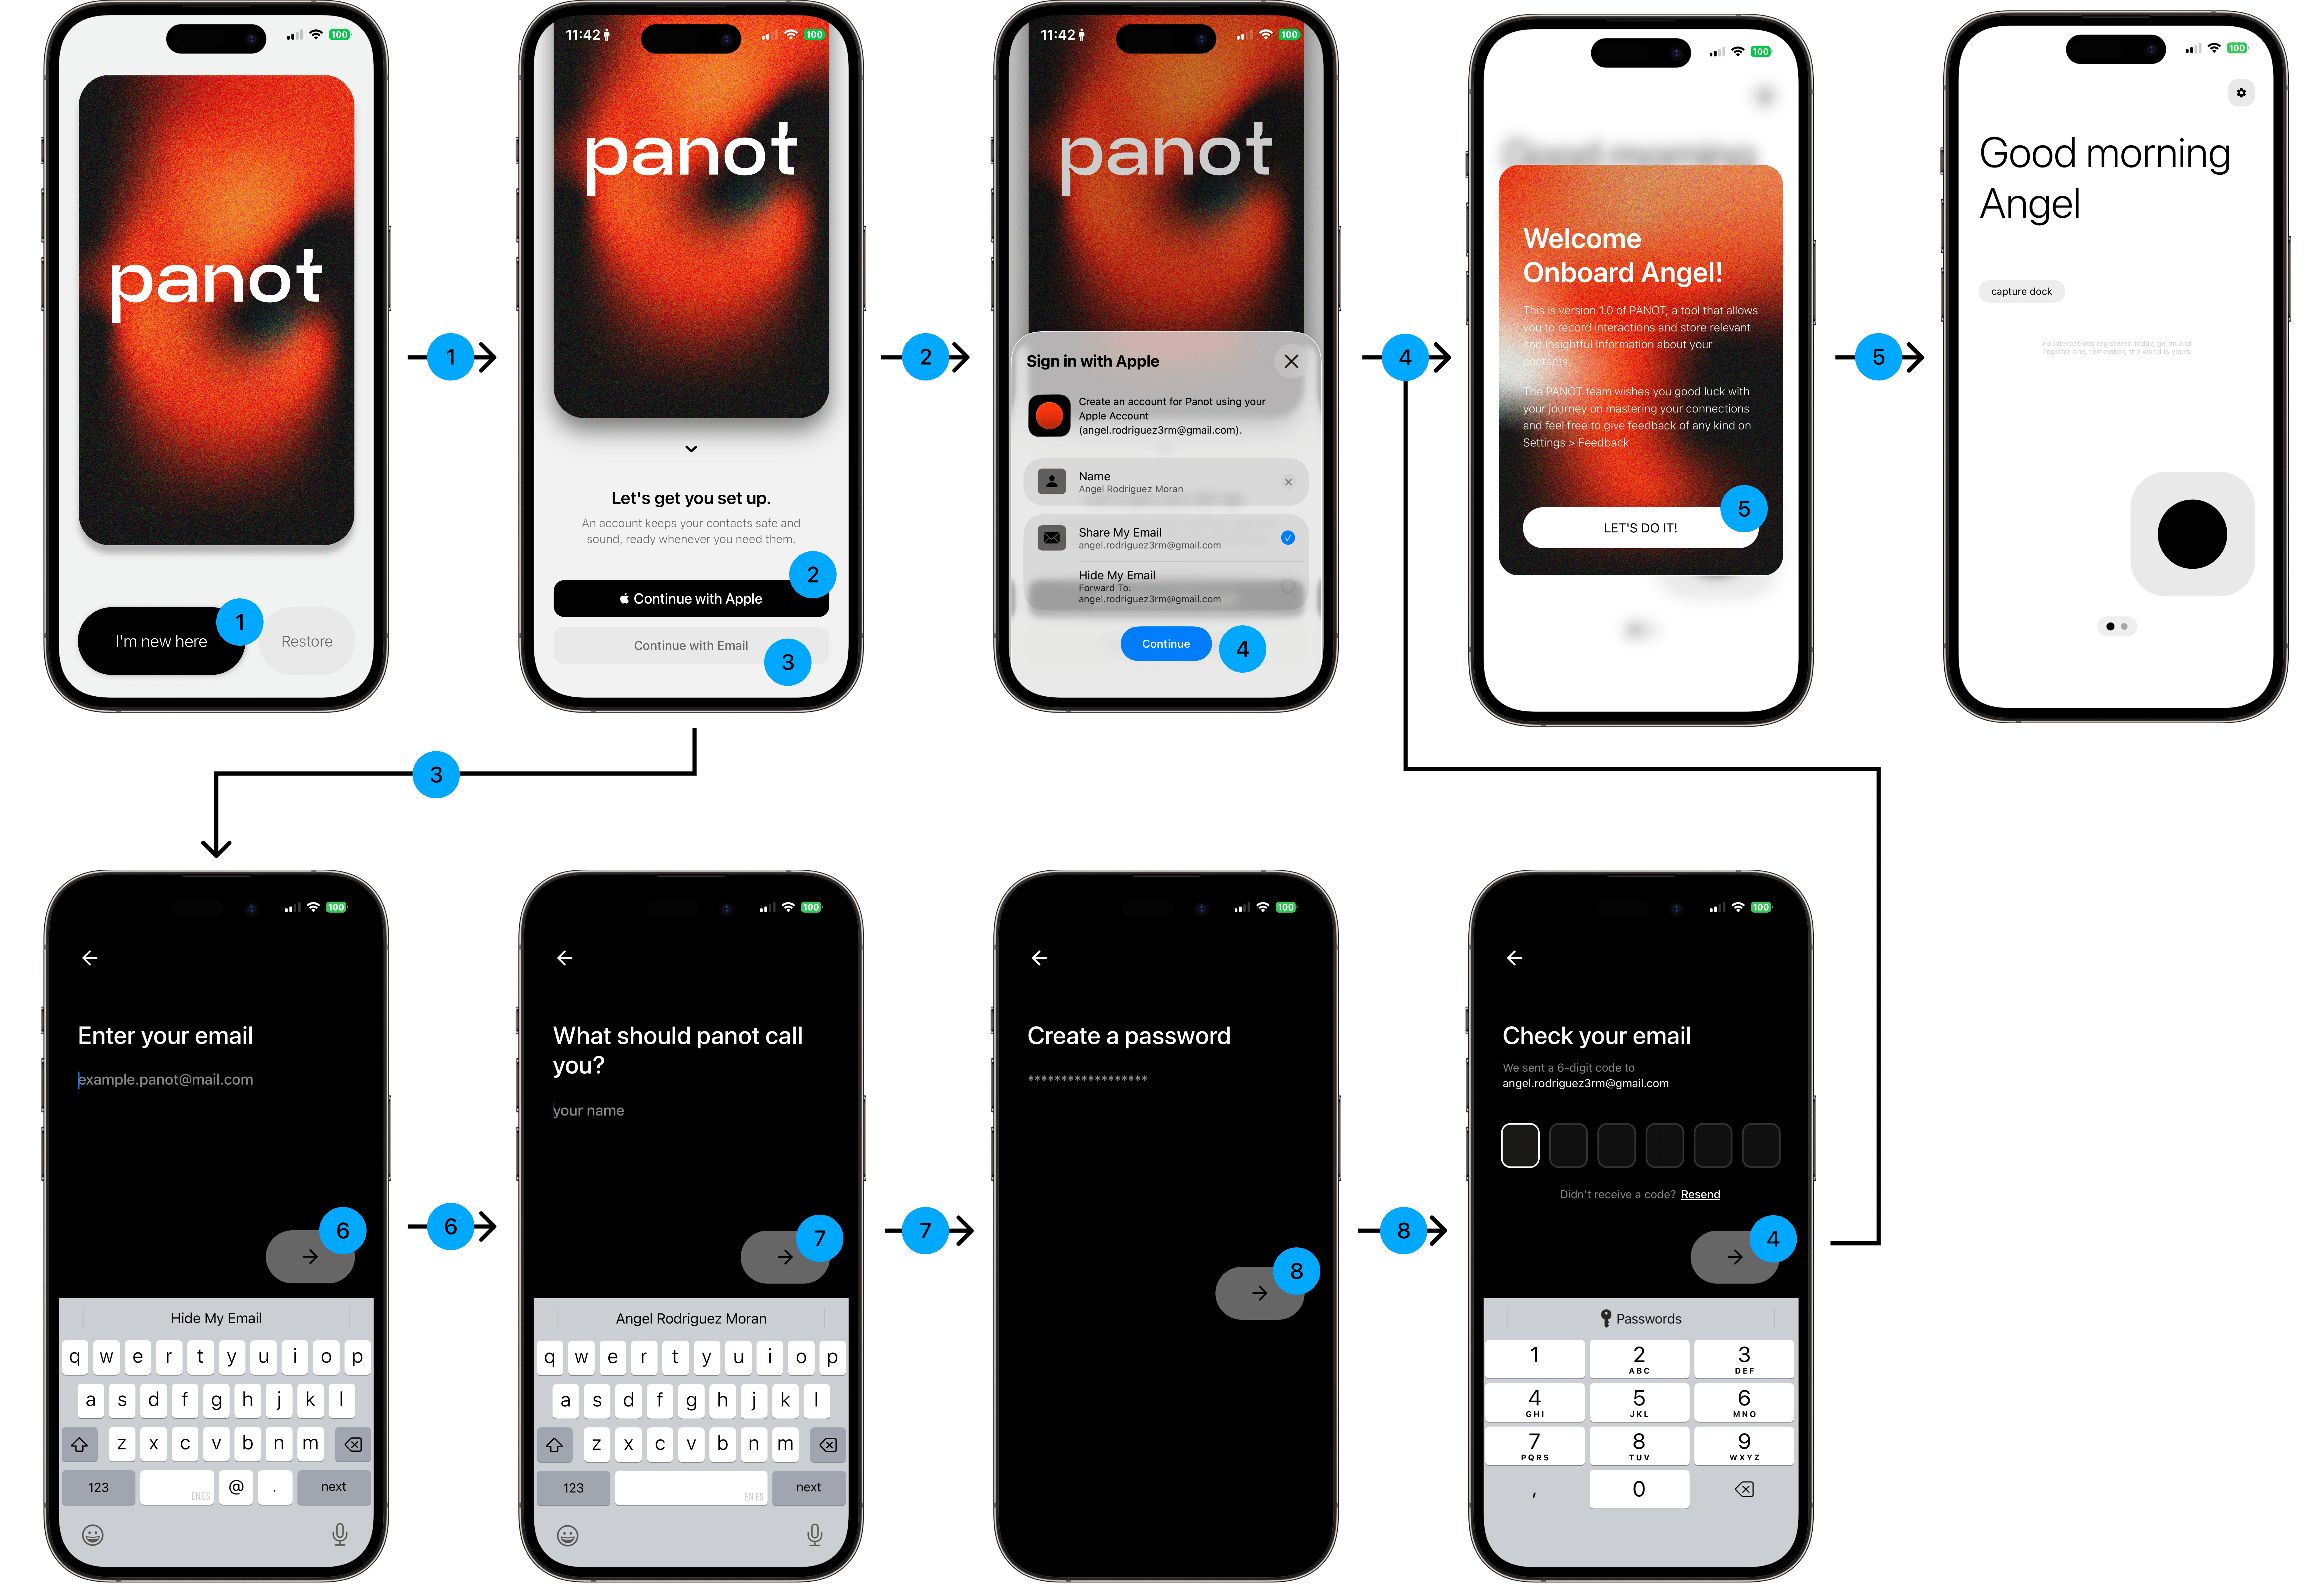
\includegraphics[width=0.8\textwidth]{figures/user-flow-onboarding.png}
    \caption{Flujo de Registro de Usuario y Onboarding}
    \label{fig:onboarding}
\end{figure}

\subsubsection{Flujo de Inicio de Sesión - \hyperref[req:HU-01]{HU-01}}

\begin{figure}[H]
    \centering
    \includegraphics[width=0.75\textwidth]{figures/user-flow-signin.png}
    \caption{Flujo de Inicio de Sesión}
    \label{fig:signin}
\end{figure}

Ambos flujos de Registro \ref{fig:onboarding} e Inicio de Sesión \ref{fig:signin} recogen la posibilidad de que el usuario use su \textit{Correo electrónico} o su \textit{Apple ID} como proveedor de autenticación.

\vspace{3.5cm}
\subsubsection{Flujo de Creación de Contacto - \hyperref[req:HU-02]{HU-02} y \hyperref[req:HU-03]{HU-03}}

El siguiente flujo de ususario abarca las tres posibilidades de creación de un contacto: creación manual (camino \textit{1 - 2 - 4 - 9}), creación con dictado (camino \textit{1 - 2 - 5 - 10 - 11}) e 
importación del contacto (camino \textit{1 - 2 - 6 - 7-  8}).

\begin{figure}[H]
    \centering
    \includegraphics[width=0.8\textwidth]{figures/user-flow-new-contact.png}
    \caption{Flujo de Creación de Contacto}
    \label{fig:new-contact}
\end{figure}

Para validar el funcionamiento de este proceso, se ha analizado la orquestación interna del sistema tras la creación del contacto \textbf{Pedro}. Como se observa en la Figura \ref{fig:trace-pedro}, 
el motor multi-agente inicia una traza de ejecución para crear el nuevo contacto con su grafo contextual correspondiente.

\begin{figure}[H]
    \centering
    \includegraphics[width=0.9\textwidth]{figures/traza-ejemplo-pedro.png}
    \caption{Traza de ejecución en LangSmith para la creación del contacto \textbf{Pedro}.}
    \label{fig:trace-pedro}
\end{figure}

El resultado es el siguiente grafo semántico (ver Figura \ref{fig:grafo-pedro}) donde el contacto no es una entrada tabular, sino el nodo central de una red de conceptos.

\begin{figure}[H]
    \centering
    \includegraphics[width=0.5\textwidth]{figures/grafo-inicial-pedro.png}
    \caption{Grafo de conocimiento resultante de la creación del contacto \textbf{Pedro}.}
    \label{fig:grafo-pedro}
\end{figure}


Posteriormente, al crear el contacto \textbf{Pepe}, el sistema activa el \textit{matching semántico} para identificar nodos comunese entre los contactos. Como se evidencia en la Figura \ref{fig:grafo-pedro-pepe-inicial}, el sistema 
ha identificado de forma autónoma que ambos tienen los nodos comunes \textbf{Universidad Complutense} y \textbf{pádel}, estableciendo una conexión relacional entre los dos contactos sin intervención del usuario.

\begin{figure}[H]
    \centering
    \includegraphics[width=0.8\textwidth]{figures/grafo-pedro-pepe.png}
    \caption{Grafo de conocimiento resultante de la creación del contacto \textbf{Pepe} y la detección de nodos comunes con el contacto \textbf{Pedro}.}
    \label{fig:grafo-pedro-pepe-inicial}
\end{figure}

\vspace{.5cm}
\subsubsection{Flujo de Grabación y Procesamiento de Interacción - \hyperref[req:HU-04]{HU-04}, \hyperref[req:HU-06]{HU-06} y \hyperref[req:HU-08]{HU-08}}

Los siguientes flujos de creación y procesamiento de una interacción que se exponene a continuación corresponden dos variantes: la primera (\hyperref[fig:new-interaction-long]{I}) corresponde a asignación de la interacción a un 
contacto previo a aceptar la creación de la interacción. Mientras que la segunda (\hyperref[fig:new-interaction-short]{II}) corresponde a la creación de una nueva interacción sin asignarla a un contacto previamente.

\begin{figure}[H]
    \centering
    \includegraphics[width=0.8\textwidth]{figures/user-flow-new-interaction-long.png}
    \caption{Flujo de Grabación y Procesamiento de Interacción (I)}
    \label{fig:new-interaction-long}
\end{figure}

\begin{figure}[H]
    \centering
    \includegraphics[width=0.8\textwidth]{figures/user-flow-new-interaction-short.png}
    \caption{Flujo de Grabación y Procesamiento de Interacción (II)}
    \label{fig:new-interaction-short}
\end{figure}

La Figura \ref{fig:grafo-pedro-pepe-nueva-interaccion} muestra el grafo tras procesar las interacciones reflejando la actualización e incorporación 
de los nuevos nodos concepto en ambos contactos.

\vspace{.5cm}
\begin{figure}[H]
    \centering
    \includegraphics[width=0.9\textwidth]{figures/grafo-pedro-pepe-ni.png}
    \caption{Grafo de conocimiento resultante de los contactos \textbf{Pepe} y \textbf{Pedro} tras procesar las nuevas interacciones.}
    \label{fig:grafo-pedro-pepe-nueva-interaccion}
\end{figure}

\newpage
\subsubsection{Flujo de Soporte y Feedback - \hyperref[req:HU-09]{HU-09}}

El siguiente flujo corresponde al envío de un ticket de soporte para un bug (camino \textit{1 - 2 - 4 - 6 - 7}) o una sugerencia (camino \textit{1 - 2 - 3 - 5 - 6 - 7}).

\begin{figure}[H]
    \centering
    \includegraphics[width=0.87\textwidth]{figures/user-flow-support.png}
    \caption{Flujo de Soporte y Feedback}
    \label{fig:support-feedback}
\end{figure}

Para cerrar el ciclo de soporte, se ha verificado la recepción de estos tickets en la base de datos. La Figura \ref{fig:db-tickets} muestra los registros reales en la tabla {\footnotesize \texttt{feedback\_tickets}} de Supabase, 
confirmando que el reporte de errores y sugerencias llega correctamente al equipo de desarrollo para su gestión.

\vspace{.5cm}
\begin{figure}[H]
    \centering
    \includegraphics[width=1\textwidth]{figures/db-feedback-tickets.png}
    \caption{Verificación de persistencia: Filas de la base de datos con los tickets de soporte enviados.}
    \label{fig:db-tickets}
\end{figure}

\subsubsection{Flujo de Configuración y Ajustes}

\begin{figure}[H]
    \centering
    \includegraphics[width=0.8\textwidth]{figures/user-flow-settings.png}
    \caption{Flujo de Configuración y Ajustes}
    \label{fig:configuracion-ajustes}
\end{figure}
\section{Verificación de Requisitos}

Una vez expuestos los resultados visuales y técnicos del sistema, se procede a la verificación formal de los requisitos definidos en la fase de análisis. Este proceso asegura que el artefacto 
desarrollado cumple con la especificación original y garantiza los niveles de calidad exigidos.

\subsection{Verificación de Requisitos Funcionales}

Para validar la funcionalidad del sistema, se ha realizado un contraste entre cada requisito funcional y la evidencia generada en los flujos de usuario. En la siguiente tabla se detalla 
el estado de cumplimiento de cada requisito, vinculándolos con los flujos de la sección anterior.

\begin{table}[H]
\centering
\scriptsize
\begin{tabularx}{\textwidth}{|l|X|c|l|}
\hline
\rowcolor[HTML]{EFEFEF} 
\textit{ID} & \textit{Descripción del Requisito} & \textit{Estado} & \textit{Evidencia / Fuente} \\ \hline
\textbf{\hyperref[req:FR-01]{FR-01}} & Registro e inicio de sesión seguro. & Logrado & Flujos \ref{fig:onboarding} y \ref{fig:signin} \\ \hline
\textbf{\hyperref[req:FR-02]{FR-02}} & Cerrar sesión del usuario de forma segura. & Logrado & Flujo \ref{fig:configuracion-ajustes} \\ \hline
\textbf{\hyperref[req:FR-03]{FR-03}} & Eliminación completa de cuenta y datos. & Logrado &  Flujo \ref{fig:configuracion-ajustes} \\ \hline
\textbf{\hyperref[req:FR-04]{FR-04}} & Creación de un contacto manualmente. & Logrado & Flujo \ref{fig:new-contact} \\ \hline
\textbf{\hyperref[req:FR-05]{FR-05}} & Importación de contactos desde agenda nativa. & Logrado & Flujo \ref{fig:new-contact} \\ \hline
\textbf{\hyperref[req:FR-06]{FR-06}} & Creación de contacto mediante dictado de voz. & Logrado & Flujo \ref{fig:new-contact}, Traza \ref{fig:trace-pedro} y Fig. \ref{fig:grafo-pedro} \\ \hline
\textbf{\hyperref[req:FR-07]{FR-07}} & Búsqueda semántica y por nombre. & Logrado & Barra de búsqueda (Flujo \ref{fig:new-contact}) \\ \hline
\textbf{\hyperref[req:FR-10]{FR-10}} & Interfaz dedicada de grabación y aceptación de permisos de hardware. & Logrado & Flujos \ref{fig:new-interaction-long} y \ref{fig:new-interaction-short} \\ \hline
\textbf{\hyperref[req:FR-11]{FR-11}} & Validación de texto transcrito previo a aceptación. & Logrado & Flujos \ref{fig:new-interaction-long} y \ref{fig:new-interaction-short} \\ \hline
\textbf{\hyperref[req:FR-12]{FR-12}} & Conversión de audio a texto en tiempo real. & Logrado & Módulo {\scriptsize \texttt{panot-speech}} \\ \hline
\textbf{\hyperref[req:FR-13]{FR-13}} & Descartar una interacción. & Logrado & Flujos \ref{fig:new-interaction-long} y \ref{fig:new-interaction-short} \\ \hline
\textbf{\hyperref[req:FR-14]{FR-14}} & Actualización del grafo semántico tras interacción. & Logrado & Figuras \ref{fig:grafo-pedro-pepe-inicial} y \ref{fig:grafo-pedro-pepe-nueva-interaccion} \\ \hline
\textbf{\hyperref[req:FR-15]{FR-15}} & Generación de relaciones (matching semántico). & Logrado & Fig. \ref{fig:grafo-pedro-pepe-nueva-interaccion} (Nodos comunes) \\ \hline
\textbf{\hyperref[req:FR-16]{FR-16}} & Envío de reportes de errores o bugs. & Logrado & Flujo \ref{fig:support-feedback} y Fig.\ref{fig:db-tickets} \\ \hline
\textbf{\hyperref[req:FR-17]{FR-17}} & Envío de propuestas de mejora o solicitudes de nuevas funcionalidades. & Logrado & Flujo \ref{fig:support-feedback} y Fig. \ref{fig:db-tickets} \\ \hline
\end{tabularx}
\caption{Tabla de verificación del cumplimiento de Requisitos Funcionales. Se han omitido los requisitos \hyperref[req:FR-08]{FR-08} y \hyperref[req:FR-09]{FR-09} que corresponden a la edición y 
eliminación de un contacto por motivos de simplicidad de la memoria.}
\label{tab:verificacion-funcional}
\end{table}


\subsection{Verificación de Requisitos No Funcionales}

[VERIFICACIÓN DE REQUISITOS NO FUNCIONALES]
\section{Discusión de Resultados}

El \acrshort{mvp} construido en este proyecto es la fase \textit{Construir} del ciclo \gls{construir-medir-aprender}. Por tanto, la discusión no es sobre si PANOT es un éxito comercial, sino sobre 
si el artefacto construido es capaz de \textit{Medir} para permitir el \textit{Aprender} de manera eficiente y segura de cara al usuario.

En primer lugar, los resultados mostrados en el \hyperref[sec:latencia]{Apéndice B.2.1} (33.2s de latencia media por operación) resultan inaceptables para una aplicación convencional. No obstante, la 
implementación de la arquitectura asíncrona (cola de trabajos) y la interfaz \textit{local-first} junto con el feedback visual de la aplicación, demuestran que el usuario no percibe esta espera como fricción. 
Esta implicación tampoco resulta alarmante, ya que el valor de PANOT no reside en la inmediatez de la respuesta de los procesamientos, sino en la liberación de la carga cognitiva de la captura.

Por otro lado, el coste medio de 0,0049 USD (resultados del \hyperref[sec:eficiencia-economica]{Apéndice B.2.2}) por operación demuestra cierta viabilidad económica ya que permite confirmar que el sistema 
puede ofrecerse bajo un modelo freemium sin riesgo de quiebra operativa inmediata.

Por último, la verificación de las políticas \acrshort{rls} (\hyperref[appendix:seguridad]{Apéndice B.1}) y la anonimización de las métricas en \textit{PostHog} (\hyperref[appendix:posthog-anonimizacion]{Apéndice B.3}) 
demuestra que es posible recolectar métricas de producto para \textit{Medir} sin comprometer la soberanía del dato del usuario. Esto permite garantizar la privacidad y seguridad del usuario desde el diseño.

\chapter{Conclusiones y Trabajo Futuro}
\label{ch:conclusiones-y-trabajo-futuro}

\section{Conclusiones Generales}

Este trabajo fin de grado ha cumplido con el objetivo general de materializar un \gls{mvp} funcional, cerrando con éxito la fase \textit{Construir} del ciclo expuesto en el libro 
\textit{The Lean Startup} \cite{ries2011lean} que ha servido como referencia y marco metodológico durante todo el desarrollo del proyecto. Además, a través del desarrollo de PANOT, 
se ha demostrado que la Inteligencia Relacional puede ser asistida tecnológicamente mediante un motor multi-agente sin sacrificar simplicidad de uso.

\noindent Respecto a los objetivos específicos:

\begin{itemize}
    \item Se ha fundamentado el cambio de paradigma del contacto tabular al grafo de conocimiento (\hyperref[o1]{O1}).
    \item Se ha implementado un motor multiagéntico (\hyperref[o2]{O2}) y una interfaz \textit{voice-first} (\hyperref[o4]{O4}) que reducen drásticamente la fricción de entrada de datos.
    \item La arquitectura \textit{local-first} (\hyperref[o3]{O3}) y los mecanismos de seguridad (\hyperref[o6]{O6}) garantizan una herramienta eficiente y privada.
    \item El sistema ha sido instrumentado y desplegado con éxito (\hyperref[o5]{O5} y \hyperref[o7]{O7}), estando ya disponible globalmente y listo para iniciar la fase de \textit{Medir}.
\end{itemize}

%%%%%%%%%%%%%%%%%%%%%%%%%%%%%%%%%%%
% APLICACIÓN DE CONOCIMIENTOS ADQUIRIDOS EN EL GRADO

\section{Aplicación de Conocimientos Adquiridos en el Grado}

[Escribir aquí la aplicación de conocimientos adquiridos en el grado]

\input{chapter6-conclusiones/3-lineas-trabajo-futuro}

\appendix

\chapter{Evidencias de Verificación de Requisitos No Funcionales}

\section{\hyperref[req:RNF-SEG-001]{RNF-SEG-001} - Seguridad}
\label{appendix:seguridad}

\begin{figure}[H]
    \centering
    \includegraphics[width=1\textwidth]{figures/rls-graph.png}
    \caption{Política RLS para las tablas \texttt{semantic\_edges} y \texttt{semantic\_nodes}.}
    \label{fig:rls-graph}
\end{figure}

\begin{figure}[H]
    \centering
    \includegraphics[width=1\textwidth]{figures/rls-interactions.png}
    \caption{Política RLS para la tabla \texttt{interactions}.}
    \label{fig:rls-interactions}
\end{figure}


\begin{figure}[H]
    \centering
    \includegraphics[width=1\textwidth]{figures/rls-profiles.png}
    \caption{Política RLS para la tabla \texttt{profiles}.}
    \label{fig:rls-profiles}
\end{figure}

\begin{figure}[H]
    \centering
    \includegraphics[width=1\textwidth]{figures/rls-contacts.png}
    \caption{Política RLS para la tabla \texttt{contacts}.}
    \label{fig:rls-contacts}
\end{figure}


\begin{figure}[H]
    \centering
    \includegraphics[width=1\textwidth]{figures/rls-workers.png}
    \caption{Política RLS para la tabla \texttt{workers}.}
    \label{fig:rls-workers}
\end{figure}

\begin{figure}[H]
    \centering
    \includegraphics[width=1\textwidth]{figures/rls-process-queue.png}
    \caption{Política RLS para la tabla \texttt{process\_queue}.}
    \label{fig:rls-process-queue}
\end{figure}

\begin{figure}[H]
    \centering
    \includegraphics[width=1\textwidth]{figures/rls-tickets.png}
    \caption{Política RLS para la tabla \texttt{feedback\_tickets}.}
    \label{fig:rls-tickets}
\end{figure}


\newpage
\section{\hyperref[req:RNF-REND-002]{RNF-REND-002} y \hyperref[req:RNF-EFI-003]{RNF-EFI-003} - Rendimiento y Eficiencia}
\label{sec:rendimiento-eficiencia}

Para validar los requisitos de rendimiento y eficiencia económica del sistema multi-agente de PANOT, se ha realizado una evaluación de carga consistente en 27 ejecuciones consecutivas del 
sistema ({\footnotesize \texttt{relational\_agent}}) utilizando transcripciones reales de longitud media (aprox. 300 palabras). Los datos de los resultados han sido extraídos de la plataforma de 
observabilidad \textit{LangSmith}.

\vspace{.5cm}
\begin{figure}[H]
    \centering
    \includegraphics[width=0.7\textwidth]{figures/lista-trazas.png}
    \caption{Lista de trazas de ejecución en LangSmith.}
    \label{fig:lista-trazas}
\end{figure}


\subsection{Análisis de Latencia - \hyperref[req:RNF-REND-002]{RNF-REND-002}}
\label{sec:latencia}

Dada la naturaleza estocástica de los modelos de lenguaje, el tiempo de respuesta ($T$) de una solicitud presentan una alta varianza debida a la carga del modelo, el tamaño de la ventana de contexto y la profundidad de la inferencia. 
Para evaluar el cumplimiento del requisito \hyperref[req:RNF-REND-002]{RNF-REND-002}, se analizan las siguientes métricas estadísticas sobre la muestra de las $n=27$ trazas:

\begin{enumerate}
    \item \textbf{Latencia End-to-End (E2E) ($T_{e2e}$):} Define el tiempo total desde el inicio del proceso hasta la respuesta final. Para cada observación $i$, se calcula como:
    \begin{equation}
        T_{e2e,i} = t_{final,i} - t_{inicio,i}
    \end{equation}

    \item \textbf{Teimpo de Respuesta Medio ($\bar{T}$):} La media aritmética de los tiempos de respuesta. Esta métrica es el indicador principal de rendimiento esperado bajo una carga constante.
    \begin{equation}
        \bar{T} = \frac{1}{n} \sum_{i=1}^{n} T_{e2e,i}
    \end{equation}

    \item \textbf{Mediana ($M$):} Representa el valor central de la muestra. En sistemas agenticos, se utiliza para neutralizar el sesgo de los valores atípicos (\textit{outliers}) provocados por la 
    latencia variable de las \acrshort{api} de terceros. Para una muestra ordenada $x_{(1)} \leq x_{(2)} \leq \ldots \leq x_{(n)}$:
    \begin{equation}
        M = \begin{cases}
            x_{((n+1)/2)} & \text{si } n \text{ es impar (nuestro caso: $n=27$)} \\[0.5em]
            \dfrac{x_{(n/2)} + x_{(n/2+1)}}{2} & \text{si } n \text{ es par}
        \end{cases}
    \end{equation}

\end{enumerate}

\subsubsection{Resultados}

\begin{figure}[H]
    \centering
    \includegraphics[width=0.9\textwidth]{figures/latencia-trazas.png}
    \caption{Gráfica de latencia por traza en LangSmith. Listado de valores de latencia ($T_{e2e}$): 28.89; 37.34; 34.37; 46.75; 34.03; 40.45; 30.48; 29.06; 30.60; 31.19; 34.84; 31.96; 35.06; 32.99; 35.42; 37.17; 28.09; 45.99; 32.48; 29.69; 34.50; 7.75; 32.07; 32.42; 31.39; 34.37; 37.60}
    \label{fig:latencia-trazas}
\end{figure}

Tras el procesamiento de la muestra (Fig. \ref{fig:lista-trazas}), los resultados arrojan una \textbf{Latencia Media ($\bar{T}$)} de \textbf{33,22 segundos} y una \textbf{Mediana ($M$)} de 
\textbf{32,99 segundos}. Ambos valores se sitúan por debajo del \textit{threshold} de \textbf{35 segundos} establecido como indicador de éxito.

\vspace{1cm}
\subsection{Análisis de Eficiencia Económica - \hyperref[req:RNF-EFI-003]{RNF-EFI-003}}
\label{sec:eficiencia-economica}

La eficiencia económica del sistema se evalúa en función del coste operativo directo por cada ejecución del sistema agéntico. Este coste está determinado por el consumo de 
recursos computacionales del procesamiento de lenguaje natural, el cual se tarifica mediante el uso de \textit{tokens} de entrada y salida. Para validar el cumplimiento 
del requisito \hyperref[req:RNF-EFI-003]{RNF-EFI-003}, se analizan las siguientes métricas sobre la muestra de las $n=27$ trazas:

\begin{enumerate}
    \item \textbf{Coste por Ejecución ($C_i$):} Representa el gasto monetario de una traza individual, derivado del volumen de información procesada ($I$: \textit{tokens} de 
    entrada, $O$: \textit{tokens} de salida) y el coste por \textit{token} del modelo ($\tau$):
    \begin{equation}
        C_i = (I_i \cdot \tau_{in}) + (O_i \cdot \tau_{out})
    \end{equation}

    \item \textbf{Coste Medio ($\bar{C}$):} El promedio aritmético del coste de todas las ejecuciones de la muestra, utilizado para proyectar la viabilidad económica a largo plazo:
    \begin{equation}
        \bar{C} = \frac{1}{n} \sum_{i=1}^{n} C_i
    \end{equation}
\end{enumerate}

\subsubsection{Resultados}

\begin{figure}[H]
    \centering
    \includegraphics[width=0.9\textwidth]{figures/coste-trazas.png}
    \caption{Gráfica de coste por traza en LangSmith. Listado de valores de coste ($C_i$) en USD: 0.0044; 0.0042; 0.0052; 0.0046; 0.0049; 0.0056; 0.0044; 0.0052; 0.0048; 0.0047; 0.0045; 0.0045; 0.0057; 0.0047; 0.0050; 0.0055; 0.0051; 0.0080; 0.0054; 0.0047; 0.0054; 0.0012; 0.0045; 0.0052; 0.0051; 0.0060; 0.0060.}
    \label{fig:coste-trazas}
\end{figure}

Tras analizar los datos de facturación de las $n=27$ trazas (Fig. \ref{fig:coste-trazas}), el \textbf{Coste Medio ($\bar{C}$)} resultante es de \textbf{\$0,0049} (aproximadamente 0,005 
unidades monetarias). Comparando este resultado con el \textit{threshold} de \textbf{0,01}, se evidencia que el sistema opera con un margen de eficiencia del 
\textbf{50\%} respecto al límite máximo permitido.


\newpage
\section{\hyperref[req:RNF-MANT-008]{RNF-MANT-008} - Mantenibilidad}
\label{appendix:posthog-metrics}

Para validar las hipótesis de valor planteadas en la sección \ref{sec:valor-hipotesis} y asegurar la mantenibilidad del sistema a través de la 
toma de decisiones basada en datos, se ha instrumentado la aplicación mediante la plataforma de analítica de producto \textit{PostHog}.

\subsubsection{Eventos de Captura}

Esta instrumentación se ha diseñado para medir el éxito y la fricción en los flujos críticos de la aplicación. Se han definido los siguientes eventos específicos que permiten monitorizar el flujo del usuario 
desde que inicia una acción hasta que esta se completa con éxito:

\vspace{1cm}
\begin{table}[H]
\scriptsize
\begin{tabularx}{\textwidth}{|l|X|}
\hline
\rowcolor[HTML]{EFEFEF} 
{\footnotesize \textit{Nombre de evento}} & {\footnotesize \textit{Descripción}} \\ \hline
{\scriptsize \texttt{START\_MANUAL\_NEW\_CONTACT}} & Inicio de creación manual de un contacto. \\ \hline
{\scriptsize \texttt{CANCEL\_MANUAL\_NEW\_CONTACT}} & Cancelación del flujo de creación manual de un contacto. \\ \hline
{\scriptsize \texttt{MANUAL\_NEW\_CONTACT\_SUCCESS}} & Contacto creado correctamente de forma manual. \\ \hline
{\scriptsize \texttt{START\_RECORDING\_NEW\_CONTACT}} & Inicio de grabación por voz para nuevo contacto. \\ \hline
{\scriptsize \texttt{EDIT\_TEXT\_RECORDING\_NEW\_CONTACT}} & Edición del texto transcrito del dictado. \\ \hline
{\scriptsize \texttt{CANCEL\_RECORDING\_NEW\_CONTACT}} & Cancelación de la creación por dictado de creación de un contacto. \\ \hline
{\scriptsize \texttt{RECORDING\_NEW\_CONTACT\_SUCCESS}} & Contacto creado correctamente por dictado. \\ \hline
{\scriptsize \texttt{START\_IMPORTING\_NEW\_CONTACT}} & Inicio de importación de un contacto. \\ \hline
{\scriptsize \texttt{IMPORTING\_NEW\_CONTACT\_SUCCESS}} & Contacto importado correctamente. \\ \hline
{\scriptsize \texttt{START\_MANUAL\_EDIT\_CONTACT}} & Inicio de edición manual de un contacto. \\ \hline
{\scriptsize \texttt{CANCEL\_MANUAL\_EDIT\_CONTACT}} & Cancelación de la edición del contacto. \\ \hline
{\scriptsize \texttt{MANUAL\_EDIT\_CONTACT\_SUCCESS}} & Contacto editado correctamente. \\ \hline
{\scriptsize \texttt{DELETE\_MANUAL\_CONTACT}} & Eliminación de un contacto. \\ \hline
{\scriptsize \texttt{VIEW\_CONTACT}} & Visualización de la ficha de un contacto. \\ \hline
{\scriptsize \texttt{START\_INTERACTION\_RECORDING}} & Inicio de grabación de una interacción (voz). \\ \hline
{\scriptsize \texttt{CANCEL\_INTERACTION\_RECORDING}} & Cancelación de la grabación de interacción. \\ \hline
{\scriptsize \texttt{EDIT\_TEXT\_RECORDING\_INTERACTION}} & Edición del texto de la interacción grabada. \\ \hline
{\scriptsize \texttt{INTERACTION\_RECORDING\_SUCCESS}} & Interacción grabada correctamente. \\ \hline
{\scriptsize \texttt{ASSIGN\_UNASSIGNED\_INTERACTION}} & Asignación de una interacción sin asignar. \\ \hline
{\scriptsize \texttt{SELECT\_CONTACT\_TO\_ASSIGN\_INTERACTION}} & Selección de contacto para asignar la interacción. \\ \hline
{\scriptsize \texttt{ASSIGN\_INTERACTION\_SUCCESS}} & Interacción asignada correctamente. \\ \hline
{\scriptsize \texttt{VIEW\_INTERACTION}} & Visualización del detalle de una interacción. \\ \hline
{\scriptsize \texttt{DELETE\_INTERACTION}} & Eliminación de una interacción. \\ \hline
{\scriptsize \texttt{MANUAL\_PROCESS\_INTERACTION}} & Procesamiento manual de una interacción. \\ \hline
\end{tabularx}
\caption{Eventos de PostHog capturados en la aplicación}
\label{tab:eventos-posthog}
\end{table}

\subsubsection{Anonimización de Datos}

En cumplimiento con los principios de \textit{Privacidad desde el Diseño}, se ha implementado una capa de abstracción en el envío de métricas 
para que se desabiliten los campos de información sensible o geolocalización del usuario. Como se observa en el siguiente fragmento de código, se han desactivado explícitamente los 
campos de \textit{GeoIP} (ciudad, país, latitud/longitud), la dirección IP, la zona horaria y la configuración de idioma local (\textit{locale}). Esta medida asegura que las 
métricas obtenidas sean puramente operacionales y anónimas.

{\scriptsize
\begin{lstlisting}[language=TypeScript, caption=Implementación de abstracción de eventos con anonimización de metadatos.]
posthog.capture(event_name, {
  $geoip_disable: true,
  $ip: "",
  $locale: false,
  $timezone: false,
  // Desactivación de todos los campos de geolocalización
  $geoip_city_name: false,
  $geoip_country_code: false,
  ...properties,
});
\end{lstlisting}}

\subsubsection{Verificación del Flujo de Datos}

La Figura \ref{fig:evidencia-posthog-stream} muestra el flujo de eventos en tiempo real capturado durante una prueba de uso. Se confirma la recepción de los eventos 
lo que permite validar que el sistema de monitorización es plenamente funcional y capaz de impulsar el ciclo de aprendizaje validado de la metodología \textit{Lean Startup} (fases \textit{Medir-Aprender}).

\vspace{.5cm}
\begin{figure}[H]
    \centering
    \includegraphics[width=.8\textwidth]{figures/posthog-event-stream.png}
    \caption{Flujo de eventos recibido en el panel de PostHog.}
    \label{fig:evidencia-posthog-stream}
\end{figure}

\end{document}
